\ifnum \aluno=1
\renewcommand\chapterillustration{abertura-taxa}
\else
\renewcommand\chapterillustration{abertura-taxa-professor}
\fi
\renewcommand\chapterwhat{Taxas de variação média e instantânea de uma função real. Tipos de crescimento e decrescimento.}
\renewcommand\chapterbecause{É bastante comum nos depararmos com taxas em nosso cotidiano, informações que tratam de taxas de natalidade e mortalidade, taxa de variação cambial, velocidade, frequência, potência, inflação, aceleração, ritmo etc. Em algum sentido a taxa de variação é a generalização da ideia de razão. Enquanto razão é a comparação entre duas medidas a taxa de variação surge quando há covariação entre duas grandezas, ou seja, quando uma pode ser expressa como função da outra. A taxa de variação, então, é uma razão que traz consigo informações sobre duas grandezas que covariam sendo uma ferramenta poderosa para a interpretação de gráficos e a consequente compreensão de diferentes fenômenos e situações que nos cercam.}

\chapter{Taxa de Variação}

\mbox{}\thispagestyle{empty}\clearpage

\thispagestyle{empty}

\begin{center}
Projeto: LIVRO ABERTO DE MATEMÁTICA

\noindent \begin{tabular}{lcccr}

\includegraphics[scale=.15]{impa}& \quad\quad& 
\includegraphics[width=3cm]{logo} & \quad\quad& 
\includegraphics[scale=.24]{obmep} 
\end{tabular}
\end{center}

\vspace*{.3cm}

Cadastre-se como colaborador no site do projeto: \url{umlivroaberto.org}

\begin{tabular}{p{.15\textwidth}p{.7\textwidth}}
Título: & Taxa de Variação\\
\\
Ano/ Versão: & 2020 / versão 1.0 de 24 de março de 2020\\
\\
Editora & Instituto Nacional de Matem\'atica Pura e Aplicada (IMPA-OS)\\
\\
Realização:& Olimp\'iada Brasileira de Matem\'atica das Escolas P\'ublicas (OBMEP)\\
\\
Produção:& Associação Livro Aberto\\
\\
Coordenação:& Fabio Simas, \\ 
			& Augusto Teixeira (livroaberto@impa.br)\\
\\
Autores: & Gladson Antunes (UNIRIO) e\\
         & Michel Cambrainha (UNIRIO) \\
\\
Revisão &  Wanderley Rezende\\
                
\\
Design: & Andreza Moreira (Tangentes Design) \\
\\
  Ilustrações: & --- \\ 
\\
Gráficos: & Tarso Caldas (Licenciando da UNIRIO)\\
\\
  Capa: & Foto do site Freepik \\
  		& shorturl.at/owJQ2 \\

\end{tabular}

\begin{figure}[b]
\begin{minipage}[l]{5cm}
\centering

{\large Licença:}

  
\includegraphics[width=3.5cm]{cc-by-sa1}
\end{minipage}\hfill
\begin{minipage}[c]{5cm}
\centering
{\large Desenvolvido por}


\includegraphics[width=2.5cm]{logo-associacao.jpg}
\end{minipage}
\begin{minipage}[r]{5cm}
\centering

{\large Patrocínio:}
  \vspace{1em}
  
\includegraphics[width=3.5cm]{itau}
\end{minipage}
\end{figure}

\mainmatter

\begin{apresentacao}
\section{Taxa de Variação}

Entendemos que o estudo de taxa de variação dará maior significado ao estudo de funções no Ensino Médio. Esta será uma oportunidade de oforecer ao estudante a possibilidade de explorar mais o caráter dinâmico que envolve o conceito de função. Reforça esse entendimento o fato de que tal característica está na essência do surgimento da noção de função. Segundo Roque:

\begin{quote}
[...] O estudo da variação por meio de leis matemáticas se deve em grante parte ao desenvolvimento da Física pós-Galileu. A ideia de uma variação em função do tempo é fundamental em seus trabalhos, onde já encontramos uma certa noção de função no sentido de uma associação entre duas grandezas que variam, dada por uma proporção geométrica. 

Úma função pode ser vista justamente como uma relação entre duas grandezas que variam. Para Descartes, essa relação devia ser algébrica, uma vez que não se associava uma grandeza Física ao tempo. Ou seja, o movimento que gera uma relação de tipo funcional deveria ser, para Descartes, de natureza geométrica, mas não física. No caso de Galileu era diferente, pois ele desejava entender o movimento físico [...]
\flushright

(Roque, 2012, p.336)
\end{quote}

A necessidade de resgatar o conceito dinâmico no estudo do conceito de função é defendida também por Rezende.

\begin{quote}
Fala-se, por exemplo, em injetividade ou sobrejetividade, mas nãoi em crescimento ou decrescimento da função, ou melhor, em quanto e como cresce/decresce o valor de uma função em relação à sua variável independente. A noção de função é estabelecida não no contexto da variabilidade, mas, em termos de uma correspondência estática entre os valores das variáveis "$x$"{}e "$y$". O gráfico de uma função é, em geral, plotado através de uma tabela de valores notáveis. As curvaturas das curvas que compões os gráficos das funções são, em geral, induzidas pelo acréscimo de mais pontos.

\flushright
(Rezendo, Pesco, Bortolossi, 2012, p. 75)
\end{quote}

Vejam que não há erro algum em estabelecer a noção de função em termos da correspondência $(x,f(x))$, de fato, é desta forma que o conceito é apresentado na maioria dos livros didáticos do ensino básico. O que queremos chamar atenção aqui é que tal apresentação, que privilegia o formato algébrico, vai na contramão da evolução histórica do conceito de função. Ainda conforma Rezendo (2012, p.75), pode-se considerar que tal abordagem representa, efetivamente, um desvio e uma limitação de natureza epistemológica do próprio conceito de função.

As atividades trazidas por este capítulo trabalham diferentes conversões de registros de representação de funções (tabela, gráfico, expressão algébrica), essa apresentação é totalmente intencional e está apoiada na teoria de registros de representação semiótica de Duval (Duval, 1993).

Este capítulo desempenhará um papel importante também para os capítulos que tratarão de Função Linear e Afim, Função Quadrática, Exponencial e Logarítimica, uma vez que nos seus respectivos capítulos retomaremos algumas das ideias aqui tratadas. Veja, por exemplo, que uma função polinomial do primeiro grau possui taxa de variação constante em qualquer intervalo do seu domínio, e tal propriedade pode ser utilizada para caracterizar esse tipo de função, uma vez que todas as outras apresentam taxas de variação não constante.

Taxa de variação é o conceito que unifica derivada, integral, taxas relacionadas e equações diferenciais. Ela conduz uma melhor compreensão de métodos de aproximação, maximização e do Teorema Fundamental do Cálculo. Nesse sentido, os conceitos introduzidos nesse capítulo apontam na direção de uma das maiores descobertas em Matemática, a derivada. No entanto, não estamos defendendo uma antecipação de conteúdo, trata-se apenas de reconhecer que o entendimento de taxa de variação é um importante requisito para a compreensão de problemas e questões do dia-a-dia. Basta ver que é bastante comum nos depararmos com informações que tratam de taxas de natalidade e mortalidade, taxa de variação cambial, velocidade, frequência, potência, inflação, aceleração, ritmo etc. Em algum sentido a taxa de variação é a generalização da ideia de razão. Enquanto a última é a comparação entre duas medidas a taxa de variação surge quando há covariação entre duas grandezas, ou seja, quando uma pode ser expressa como função da outra. A taxa de variação, então, é uma razaão que traz consigo informações sobre duas grandezas que covariam. É bastante comum os estudantes confundirem razão com taxa, por isso recomendamos abordar esse ponto com a turma chamando atenção para a diferença entre um conceito e o outro. Uma \textit{razão} é o quociente que resulta da comparação entre duas medidas relacionadas entre si, quando as grandezas envolvidas são de natureza distintas, chamamos essa razão de \textit{taxa}. Assim, toda taxa é uma razão, mas o contrário nem sempre é verdade.

Stump (2001, p.87) coduziu um estudo para examinar como estudantes norte americanos do ensino médio compreendem a inclinação de uma reta. Os alunos foram apresentados a várias tarefas envolvendo o conceito de inclinação em seis situações. O estudo sugeriu uma lacuna na compreensão dos alunos sobre a inclinação como uma medida da taxa de variação e ujma compreensão limitada da inlcinação como uma medida do declive. Segundo o autor, este estudo implica que "a instrução deve ser focada em ajudar os alunos a estabelecer conexões entre taxas envolvendo tempo, taxas envolvendo outras variáveis e representações gráficas dessas relações". Acreditamos que as atividades propostas no capítulo apontam exatamente nessa direção. Optamos por não tratar aqui de maneira mais formal a ideia de inclinação da reta e coeficiente angular. Esta discussão ficará reservada ao capítulo de função afim.

Este capítulo tem início com uma seção "\textit{Explorando}", na qual são apresentadas uma série de atividades inspiradas em (André, 2008) e (Swan, 1982), que tratam de maneira intuitiva sobre diferentes maneiras de crescimento de uma função: lento, uniforme e rápico. Na seção "\textit{Organizando}", a taxa de variação é apresentada como uma medida de "rapidez"{} média da variação. Para além disso, é consolidade um vocabulário visando a descrição do gráfico de uma função por meio de termos como: cresce/decresce uniformemente, cresce/decresce lentamente, cresce/decresce rapidamente. Na seção "\textit{Praticando}"{}, o estudante terá a oportunidade de exercitar os conceitos recém-introduzidos em uma série de atividades em que situações cotidianas são exploradas à luz da linguagem e novos conceitos aprendidos. Por fim, o capítulo é encerrado com uma seção "\textit{Para Saber Mais}", na qual é apresentada a noção de taxa de variação instantânea como o limite das taxas de variações médias.
\end{apresentacao}

\def\currentcolor{session1}
\clearmargin
\begin{objectives}{A água está subindo}
{
\begin{itemize}

\item  Associar uma situação real a uma representação gráfica.

\item Diferenciar situações de crescimento, identificando quando o gráfico pode ser uma linha reta – taxa de variação constante (parte I) e quando não (parte II).

\item Diferenciar entre situações em que há taxa de variação constante (parte III).

\end{itemize}
}{1}{2}
\end{objectives}
\marginpar{\vspace{-2em}}
\begin{sugestions}{A água está subindo}
{
\begin{itemize}
\item Considere realizar essa atividade em grupo, principalmente em turmas maiores. Essa pode ser uma estratégia interessante para dar oportunidade para que os estudantes, em grupos, exponham suas impressões e argumentos.

\item Na parte I espera-se que os estudantes descartem rapidamente o gráfico decrescente. Certifique-se de que as justificativas contenham elementos suficientes que permitam diferenciar entre os dois gráficos crescentes.
\item Podem aparecer respostas imprecisas do tipo: "o recipiente tem os lados retos". Peça aos estudantes que sejam o mais específicos possível.
\item Não faz parte dos objetivos dessa atividade que os estudantes encontrem as fórmulas que fornecem as alturas em função do tempo.
\item Na parte III, conduza os estudantes a perceber que há uma relação decrescente entre o raio do cilindro e a taxa de variação (quanto menor o raio, maior a inclinação da reta). De fato, a taxa de variação é inversamente proporcional ao quadrado do raio.
\end{itemize}
}{1}{2}
\end{sugestions}
\clearmargin
\marginpar{\vspace{.5em}}

\begin{answer}{A água está subindo}
{
\textbf{(Parte I)}: Gráfico (II). O reservatório tem a forma de um cilíndro e a água entre a uma vazão constante.

\textbf{(Parte II)}: Gráfico (II). Devido a forma de cone do reservatório, inicialmente a coluna de água sobe mais rapidamente. Posteriormente, como a vazão de entrada de água no recipiente permanece constante durante todo o tempo, a altura da coluna sobe mais lentamente.

\textbf{(Parte III)}: A coluna de água subirá mais rapidamente no reservatório mais estreito e mais lentamente no reservatório mais largo. Dessa forma, o reservatório A está associado ao gráfico (I), o B ao gráfico (III) e o C ao gráfico (II).
}{1}
\end{answer}
\begin{objectives}{A água continua subindo}
{
\begin{itemize}

\item Registrar em palavras diversas situações que são descritas por funções crescentes, especificando mudanças de comportamento. 

\end{itemize}
}{1}{1}
\end{objectives}
\begin{sugestions}{A água continua subindo}
{
\begin{itemize}
\item Considere realizar essa atividade em grupo, principalmente em turmas maiores. Essa pode ser uma estratégia interessante para dar oportunidade para que os estudantes, em grupos, exponham suas impressões e argumentos.
\item Após os estudantes realizarem as análises, discuta com eles sobre a necessidade de se ter uma maneira sistemática de diferenciar as diversas maneiras que se pode ter um gráfico crescente.
\item Estimule-os a pensar em outras situações em que há variações similares ou situações análogas em que haja decrescimento.
\item Certifique-se que todos os estudantes compreendem o significado de "vazão constante", isto é, que o volume de água por unidade de tempo que entra em cada um dos recipientes é constante.
\item Aqui a palavra uniformemente deve ser interpretada a partir do senso comum: aquilo
que não tem variação ou mudança. Mais adiante será apresentada uma definição
precisa para o que devemos entender como crescimento/decrescimento uniforme.
\end{itemize}
}{1}{1}
\end{sugestions}
\clearmargin
\marginpar{\vspace{.5em}}
\begin{answer}{A água continua subindo}
{
Admitindo que a água entra a uma taxa constante em cada um dos recipientes, podemos descrever a maneira como a altura da coluna de água varia com o tempo da seguinte forma:

% \setlength\abovetabulinesep{2mm}
\begin{tabular}{|>{\centering\vspace{.5em}}m{.15\linewidth}<{\vspace{-.5em}}|>{\centering}m{.6\linewidth}|>{\centering}m{.125\linewidth}|}
% \endfirsthead
\hline
\tcolor{Figura} \vspace{.75em} & \tcolor{Descrição} & \tcolor{Gráfico} \tabularnewline
\begin{tikzpicture}[scale=.3]
\vspace{1em}
\draw (-3,0) -- (0,-6);
\draw (3,0) -- (0,-6);
\draw [fill=white] (0,0) ellipse [x radius=3,y radius=1];

\end{tikzpicture}
\vspace{.1em} 
& No início a coluna de água subirá rapidamente, no meio estará subindo mais lentamente e na parte final mais lentamente ainda. & (II) \tabularnewline
\hline
\begin{tikzpicture}[scale=.3]

\draw (-3,0) -- (0,6);
\draw (3,0) -- (0,6);

\draw [fill=white, dashed] (0,0) ellipse [x radius=3,y radius=1];
\clip (-3,0) rectangle (3,-1);
\draw [fill=white] (0,0) ellipse [x radius=3,y radius=1];

\end{tikzpicture}

& No início a coluna de água subirá lentamente, no meio estará subindo mais rapidamente e na parte final mais rapidamente ainda. & (V) \tabularnewline
\hline
\begin{tikzpicture}[scale=.3]

\draw (-2,0) -- (-2,5+2/3);
\draw (2,0) -- (2,5+2/3);

\draw [fill=white] (0,5+2/3) ellipse [x radius=2,y radius=2/3];

\draw [fill=white, dashed] (0,0) ellipse [x radius=2,y radius=2/3];
\clip (-3,0) rectangle (3,-1);
\draw [fill=white] (0,0) ellipse [x radius=2,y radius=2/3];


\end{tikzpicture}

& A altura da água subirá de maneira uniforme, com velocidade constante & (VI) \tabularnewline
\hline
\begin{tikzpicture}[scale=.3]

\draw (-1.5,0) .. controls (-3,1.5) and (-3,3.5) .. (-1.5,5+2/3);
\draw (1.5,0) .. controls (3,1.5) and (3,3.5) .. (1.5,5+2/3);

\draw [fill=white] (0,5+2/3) ellipse [x radius=1.5,y radius=2/3*3/4];

\draw [fill=white, dashed] (0,0) ellipse [x radius=1.5,y radius=2/3*3/4];
\clip (-3,0) rectangle (3,-1);
\draw [fill=white] (0,0) ellipse [x radius=1.5,y radius=2/3*3/4];


\end{tikzpicture}

& No início a altura de coluna subirá mais rapidamente, ficando cada vez mais lenta até chgar à metade do recipiente. Daí em diante, de maneira simétrica, voltará a acelerar. & (III) \tabularnewline\hline
\begin{tikzpicture}[scale=.3]

\draw (-2,0) -- (2,5+2/3);
\draw (2,0) -- (-2,5+2/3);

\draw [fill=white] (0,5+2/3) ellipse [x radius=2,y radius=2/3];

\draw [fill=white, dashed] (0,0) ellipse [x radius=2,y radius=2/3];
\clip (-3,0) rectangle (3,-1);
\draw [fill=white] (0,0) ellipse [x radius=2,y radius=2/3];


\end{tikzpicture}

& No início a altura da coluna de água subirá lentamente, ficando cada vez mais rápida até chegar à metade do recipiente. Daí em diante, de maneira simétrica, voltará a descelerar. & (IV) \tabularnewline
\hline
\begin{tikzpicture}[scale=.3]

\draw (-2,0) .. controls (-1,1.5) and (-1,3.5) .. (-2,5+2/3);
\draw (2,0) .. controls (1,1.5) and (1,3.5) .. (2,5+2/3);

\draw [fill=white] (0,5+2/3) ellipse [x radius=2,y radius=2/3];

\draw [fill=white, dashed] (0,0) ellipse [x radius=2,y radius=2/3];
\clip (-3,0) rectangle (3,-1);
\draw [fill=white] (0,0) ellipse [x radius=2,y radius=2/3];


\end{tikzpicture}

& Comportamento similar ao anterior, contudo, as diferenças de velocidade não são tão perceptíveis. Pode funcionar como um "meio termo"{} entre o anterior e o cilíndro. & (I) \tabularnewline
\hline
\end{tabular}
}{1}
\end{answer}
\begin{objectives}{Uma viagem de carro}
{
\begin{itemize}

\item Interpretar, em uma situação concreta, o conceito de velocidade média e suas particularidades.

\item Representar graficamente (tabela e sistema de coordenadas) as informações do problema.

\end{itemize}
}{1}{1}
\end{objectives}
\marginpar{\vspace{-2em}}
\begin{sugestions}{Uma viagem de carro}
{
\begin{itemize}
\item A escolha dessa atividade se deu pelo fato de podermos usar o conceito de velocidade
média (que é mais intuitivo e que o estudante já teve contato na disciplina de Física)
como base para a generalização de taxa de variação média de uma função qualquer.
\end{itemize}
}{1}{1}
\end{sugestions}
\begin{answer}{Uma viagem de carro}
{
\begin{enumerate}
\item \adjustbox{valign=t}{
\centering
\begin{tabu} to \textwidth{|c|c|c|}
\hline
\thead
Horário & \makecell{Tempo decorrido \\ desde a partida (h)} & \makecell{Distância percorrida \\ (km)} \\
\hline
& $t$ & $d(t)$ \\
\hline
12h & 0 & 0 \\
\hline
14h & 2 & 140 \\
\hline
14h30 & 2.5 & 140 \\
\hline
16h & 4 & 260 \\
\hline
16h30 & 4.5 & 260 \\
\hline
18h & 6 & 410 \\
\hline
\end{tabu}
}
\vspace{1em}
\begin{figure}[H]
\centering
\begin{tikzpicture}[scale=1.25, every node/.style={black},every path/.style={black}]

\draw [gray!30, step=.25] (0,0) grid (7.25,5);
\draw [gray!70] (0,0) grid (7.25,5);
\draw [->] (0,0) -- (7.25,0) node [below, shift={(0,-.5)}, pos=.82] {tempo desde a partida (h)};
\draw [->] (0,0) -- (0,5) node [pos=.75,above, rotate=90, shift={(-1,1)}] {distância percorrida (km)};
\foreach \x in {1,...,7} \node [below] at (\x,0) {\x};
\foreach \x in {1,...,4} \node [left] at (0,\x) {\x00};
\node [below left] at (0,0) {0};

\coordinate (a) at (0,0);
\coordinate (b) at (2,1.4);
\coordinate (c) at (2.5,1.4);
\coordinate (d) at (4,2.6);
\coordinate (e) at (4.5,2.6);
\coordinate (f) at (6,4.1);

\foreach \x in {a,b,c,d,e,f} \fill [\tikzcolor] (\x) circle (2pt);

\draw [dashed, \tikzcolor] (a) -- (b) -- (c) -- (d) -- (e) -- (f);
\end{tikzpicture}
\end{figure}
\end{enumerate}
}{1}
\end{answer}
\begin{answer}{Uma viagem de carro}
{
\begin{enumerate}\setcounter{enumi}{1}
\item Que, em média, a cada hora a distância percorrida foi de $51{,}5$ km. Ou que se tivesse sido mantida uma velocidade constante ao longo de toda viagem (sem paradas) esse deveria ser o valor para se chegar ao mesmo tempo no destino.

\item $\displaystyle\frac{\Delta d}{\Delta t}= \frac{140}{2}=70\frac{km}{h}$. O valor da velocidade média neste trecho é maior que o anterior. Em média, o carro andou mais rápido durante a primeira parte da viagem do que na viagem toda, fazendo $70$ km a cada hora.

\item Será menor, pois o carro passou 30 minutos parado, o que diminui a velocidade média. Em termos da conta, mantém-se o numerador e aumenta-se o denominador, gerando um número menor.

\clearpage
\item \adjustbox{valign=t}{
\begin{minipage}{\linewidth}
\setlength\tabcolsep{2.5pt}
\setlength\tabulinesep{2.5pt}
\begin{tabu} to \textwidth{|c|c|}
\hline
\thead
Intervalo de tempo $\bm{[a,b]}$ & Velocidade média $\displaystyle\bm{\frac{\Delta d}{\Delta t}=\frac{d(b)-d(a)}{b-a}}$\\
\hline
$[0,2]$ & $\displaystyle\frac{\Delta d}{\Delta t}=\frac{140}{2}=70 km/h$ \\
\hline
$[2,2.5]$ & $\displaystyle\frac{\Delta d}{\Delta t}=\frac{0}{0{,}5}=0 km/h$ \\
\hline
$[2.5,4]$ & $\displaystyle\frac{\Delta d}{\Delta t}=\frac{120}{1{,}5}=80 km/h$ \\
\hline
$[4,4.5]$ & $\displaystyle\frac{\Delta d}{\Delta t}=\frac{0}{0{,}5}=0 km/h$ \\
\hline
$[4.5,6]$ & $\displaystyle\frac{\Delta d}{\Delta t}=\frac{150}{1{,}5}=100 km/h$ \\
\hline
\end{tabu}
\end{minipage}
}

\end{enumerate}
}{1}
\end{answer}

\explore{}

\begin{figure}[H]
\centering
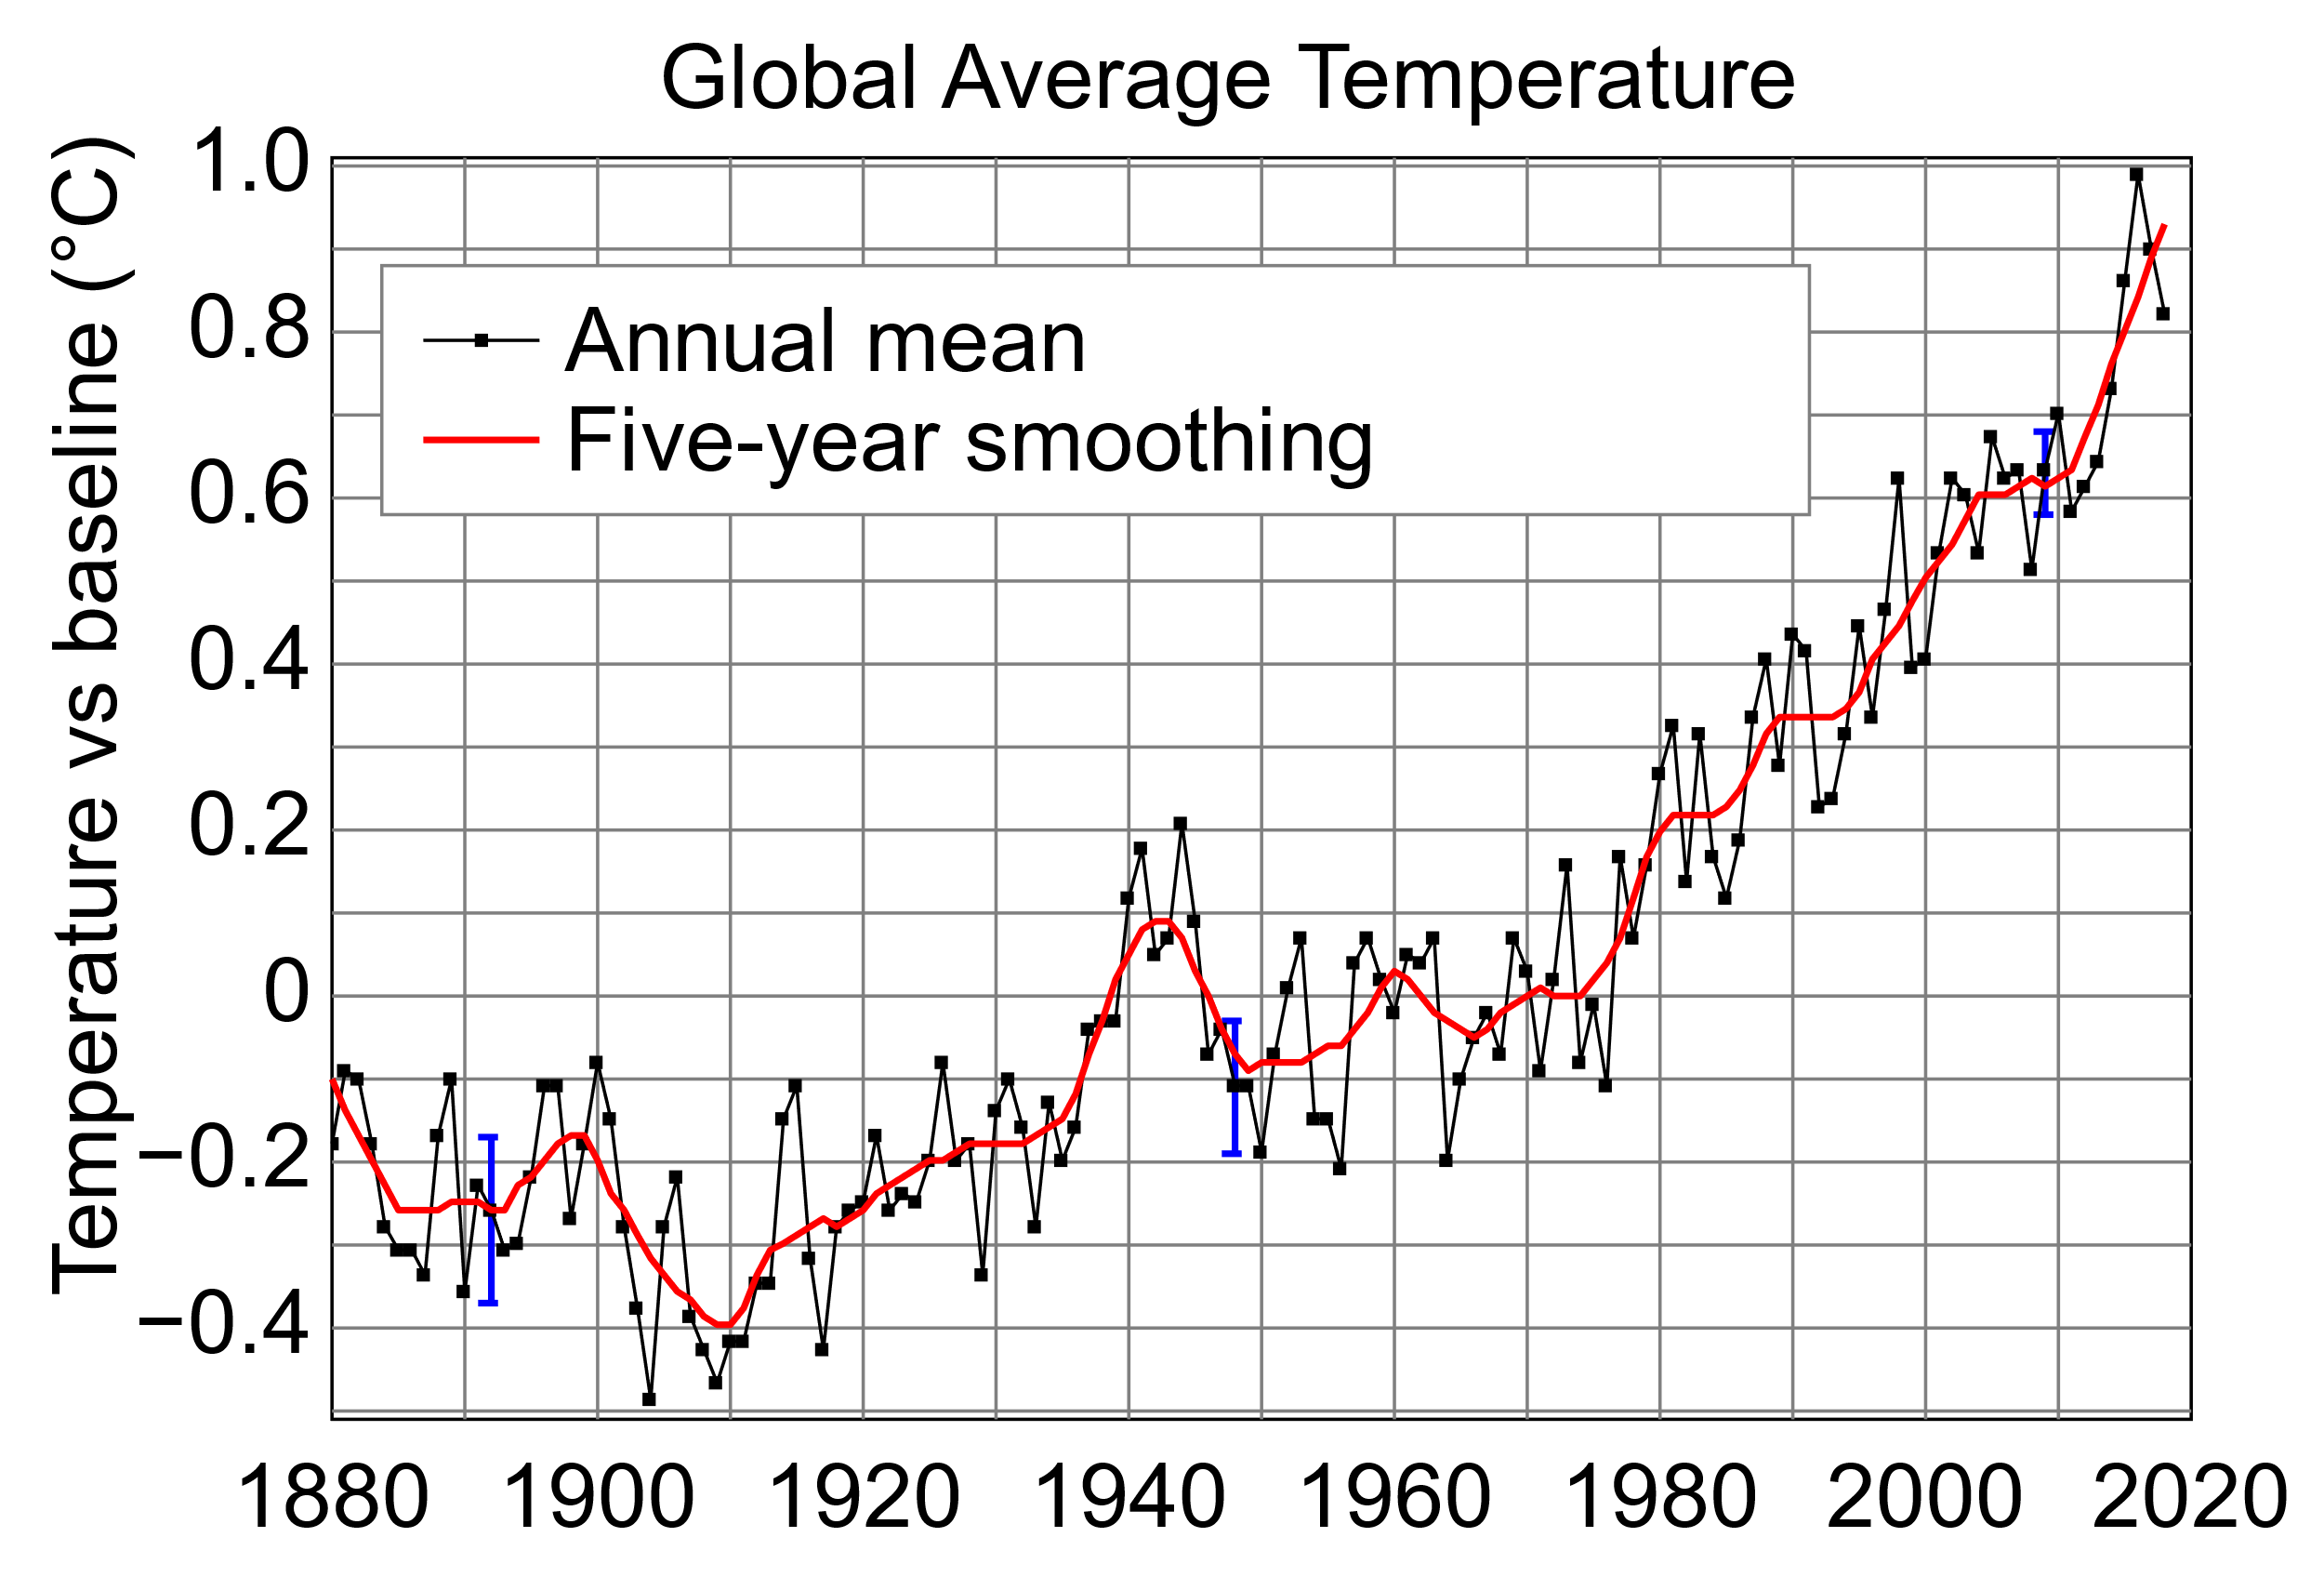
\includegraphics[width=250bp]{taxa-explore-1-1}

\caption{Por \href{http://data.giss.nasa.gov/gistemp/graphs/}{NASA Goddard Institute for Space Studies}}
\label{}
\end{figure}

A comparação está nas bases da matemática. Ela é fundamental para estabelecer os processos de contagem, de medida, para definir o conceito de número, também está presente nas ideias de razão e de proporção bem como em diversos outros contextos. No estudo das funções, quando estamos interessados em grandezas que variam conjuntamente, podemos usar a comparação para quantificar essas variações. Por exemplo, ao afirmarem que a temperatura média global está aumentando mais rapidamente agora que nos últimos anos, os cientistas fazem uso de uma ferramenta matemática que serve para medir esse crescimento: a taxa de variação. Ela serve especialmente para indicar de que maneira, ou a que velocidade, uma grandeza varia em relação a outra. 

Um investidor da bolsa de valores precisa estar bem atento às taxas de variação do preço das ações para tomar as melhores decisões sobre compra e venda. Quando os preços das ações que ele possui mostram uma tendência a crescer mais rapidamente, é hora de começar a pensar em negociá-las. Para um biólogo que estuda populações é interessante conhecer a taxa de variação do número de indivíduos por unidade de tempo. Para um biomédico, conhecer a taxa de variação da quantidade de determinado medicamento na corrente sanguínea pode indicar a efetividade de um medicamento. Para um cientista social, a taxa de variação do número de encarcerados no país pode indicar se uma determinada política pública na área de segurança pública precisa ou não ser discutida. Neste capítulo, vamos introduzir e explorar esse conceito em diversos contextos. 

Contudo a discussão não se restringirá somente a este capítulo, a taxa de variação voltará a aparecer diversas outras vezes neste livro.

\clearpage
\begin{task}{A água está subindo}

\textbf{Parte I} Um reservatório cilíndrico de altura $h$ (em cm), com capacidade máxima de $100 \ell$, encontra-se vazio. Para enchê-lo, abriu-se uma torneira que despeja $2\ell$ de água por minuto.

\begin{figure}[H]
\centering
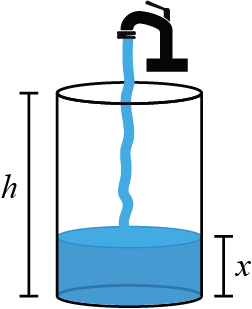
\includegraphics[width=100bp]{taxa-ativ-1-1}

%\caption{}
\label{}
\end{figure}

Qual dos gráficos seguintes expressa corretamente a variação da altura $x$ da coluna de água em função do tempo $t$? Explique.

\setlength{\columnsep}{0pt}
\begin{multicols}{3}
\begin{enumerate}[label=(\Roman*)]
\item
\adjustbox{valign=t}{\begin{tikzpicture}[scale=.5,baseline=(current bounding box.north)]

\draw [->] (-.5,0) -- (6,0) node [below ] {$t(min)$};
\draw [->] (0,-.5) -- (0,3.5) node [right] {$x(cm)$};
\draw [dashed] (0,3) -- (4,3) -- (4,0);
\node [left] at (0,3) {$h$};
\node [below left] at (0,0) {$0$};
\node [below] at (4,0) {$50$};

\draw [thick] (0,0) parabola (4,3);
\end{tikzpicture}}

\item
\adjustbox{valign=t}{\begin{tikzpicture}[scale=.5,baseline=(current bounding box.north)]

\draw [->] (-.5,0) -- (6,0) node [below ] {$t(min)$};
\draw [->] (0,-.5) -- (0,3.5) node [right] {$x(cm)$};
\draw [dashed] (0,3) -- (4,3) -- (4,0);
\node [left] at (0,3) {$h$};
\node [below left] at (0,0) {$0$};
\node [below] at (4,0) {$50$};

\draw [thick] (0,0) -- (4,3);
\end{tikzpicture}}


\item
\adjustbox{valign=t}{\begin{tikzpicture}[scale=.5,baseline=(current bounding box.north)]

\draw [->] (-.5,0) -- (6,0) node [below ] {$t(min)$};
\draw [->] (0,-.5) -- (0,3.5) node [right] {$x(cm)$};
\draw [dashed] (0,3) -- (4,3) -- (4,0);
\node [left] at (0,3) {$h$};
\node [below left] at (0,0) {$0$};
\node [below] at (4,0) {$50$};

\draw [thick] (0,3) -- (4,0);
\end{tikzpicture}}
\end{enumerate}
\end{multicols}

\textbf{Parte II} Um reservatório cônico de altura $h$ (em cm), com capacidade máxima de $100\ell$, encontra-se vazio e posicionado com o vértice para baixo, conforme mostra a figura. Para enchê-lo, abriu-se uma torneira que despeja $2\ell$ de água por minuto.

\begin{figure}[H]
\centering
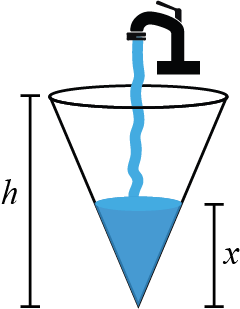
\includegraphics[width=100bp]{taxa-ativ-1-3}

%\caption{}
\label{}
\end{figure}

Qual dos gráficos seguintes expressa corretamente a variação da altura $x$ da coluna de água em função do tempo $t$? Explique.

\setlength{\columnsep}{0pt}
\begin{multicols}{3}
\begin{enumerate}[label=(\Roman*)]
\item \adjustbox{valign=t}{
\begin{tikzpicture}[scale=.5,baseline=(current bounding box.north)]

\draw [->] (-.5,0) -- (6,0) node [below ] {$t(min)$};
\draw [->] (0,-.5) -- (0,3.5) node [right] {$x(cm)$};
\draw [dashed] (0,3) -- (4,3) -- (4,0);
\node [left] at (0,3) {$h$};
\node [below left] at (0,0) {$0$};
\node [below] at (4,0) {$50$};

\draw [thick] (0,0) parabola (4,3);
\end{tikzpicture}}

\item
\adjustbox{valign=t}{\begin{tikzpicture}[scale=.5,baseline=(current bounding box.north)]

\draw [->] (-.5,0) -- (6,0) node [below ] {$t(min)$};
\draw [->] (0,-.5) -- (0,3.5) node [right] {$x(cm)$};
\draw [dashed] (0,3) -- (4,3) -- (4,0);
\node [left] at (0,3) {$h$};
\node [below left] at (0,0) {$0$};
\node [below] at (4,0) {$50$};

\draw [thick] (4,3) parabola (0,0);
\end{tikzpicture}}


\item
\adjustbox{valign=t}{\begin{tikzpicture}[scale=.5,baseline=(current bounding box.north)]

\draw [->] (-.5,0) -- (6,0) node [below ] {$t(min)$};
\draw [->] (0,-.5) -- (0,3.5) node [right] {$x(cm)$};
\draw [dashed] (0,3) -- (4,3) -- (4,0);
\node [left] at (0,3) {$h$};
\node [below left] at (0,0) {$0$};
\node [below] at (4,0) {$50$};

\draw [thick] (0,0) -- (4,3);
\end{tikzpicture}}
\end{enumerate}
\end{multicols}

\textbf{PARTE III} Os recipientes cilíndricos $A,B, \text{ e } C$, que têm altura $h$ raios da base respectivamente iguais a $r,2r$ e $3r$, estão vazios. As torneiras que os abastecem estão igualmente reguladas para despejar o mesmo número de litros de água por minuto.

\begin{figure}[H]
\centering
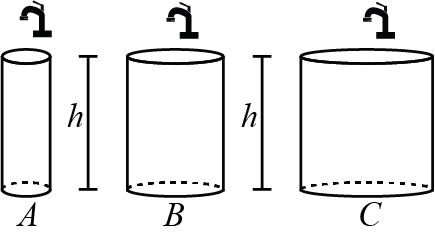
\includegraphics[width=150bp]{taxa-ativ-1-5}

%\caption{}
\label{}
\end{figure}

Os gráficos mostram a varação da altura $x$ da coluna de água em função to tempo $t$. Associe cada recipiente ao gráfico correspondente a ele e justifique suas escolhas.

\centering\setlength\tabcolsep{0pt}
% \begin{enumerate}
\begin{tabular}{m{4cm} m{6cm} m{5.5cm}}
\begin{enumerate}[label=(\Roman*)]\setcounter{enumi}{0}
\item\adjustbox{valign=t}{\begin{tikzpicture}[scale=.25,baseline=(current bounding box.north)]

\draw [->] (-.5,0) -- (3,0) node [below right] {$t(min)$};
\draw [->] (0,-.5) -- (0,5) node [right] {$x(cm)$};
\draw [dashed] (0,4) -- (2,4) -- (2,0);
\node [left] at (0,4) {$h$};
\node [below left] at (0,0) {$0$};
\node [below] at (2,0) {$b$};

\draw [thick] (0,0) -- (2,4);
\end{tikzpicture}}
\end{enumerate}

&
\hspace{0cm}
\begin{enumerate}[label=(\Roman*)]\setcounter{enumi}{1}
\item\adjustbox{valign=t}{\begin{tikzpicture}[scale=.25,baseline=(current bounding box.north), xscale=.6]

\draw [->] (-.5,0) -- (19,0) node [below right] {$t(min)$};
\draw [->] (0,-.5) -- (0,5) node [right] {$x(cm)$};
\draw [dashed] (0,4) -- (18,4) -- (18,0);
\node [left] at (0,4) {$h$};
\node [below left] at (0,0) {$0$};
\node [below] at (18,0) {$9b$};

\draw [thick] (0,0) -- (18,4);
\end{tikzpicture}}
\end{enumerate}


&
\begin{enumerate}[label=(\Roman*)]\setcounter{enumi}{2}
\item\adjustbox{valign=t}{\begin{tikzpicture}[scale=.25,baseline=(current bounding box.north), ]

\draw [->] (-.5,0) -- (9,0) node [below right] {$t(min)$};
\draw [->] (0,-.5) -- (0,5) node [right] {$x(cm)$};
\draw [dashed] (0,4) -- (8,4) -- (8,0);
\node [left] at (0,4) {$h$};
\node [below left] at (0,0) {$0$};
\node [below] at (8,0) {$4b$};

\draw [thick] (0,0) -- (8,4);
\end{tikzpicture}}
\end{enumerate}\\

\end{tabular}
\end{task}

\begin{task}{A água continua subindo}

\textbf{Parte I} Suponha que os diversos reservatórios abaixo têm a mesma capacidade, a mesma altura e que em cada um deles a água entra a uma vazão constante. Analisando a forma de cada um dos reservatórios, descreva de que maneira a altura varia em função do tempo no início, meio e fim do processo. Use, quando necessário, as palavras \textbf{lentamente}, \textbf{rapidamente} e \textbf{uniformemente}. (Gravina, 1992)\footnote{GRAVINA, M. Um estudo de funções. Revista do Professor de Matemática, n° 20, SBM, pp. 33 –38, 1992}.

\setlength\abovetabulinesep{2mm}
\begin{longtabu} to \textwidth{|c|@{\hspace{0.8\textwidth}}|}
\endfirsthead
\hline
\begin{tikzpicture}[scale=.3]

\draw (-3,0) -- (0,-6);
\draw (3,0) -- (0,-6);
\draw [fill=white] (0,0) ellipse [x radius=3,y radius=1];

\end{tikzpicture}\\
\hline
\begin{tikzpicture}[scale=.3]

\draw (-3,0) -- (0,6);
\draw (3,0) -- (0,6);

\draw [fill=white, dashed] (0,0) ellipse [x radius=3,y radius=1];
\clip (-3,0) rectangle (3,-1);
\draw [fill=white] (0,0) ellipse [x radius=3,y radius=1];

\end{tikzpicture}\\
\hline
\begin{tikzpicture}[scale=.3]

\draw (-2,0) -- (-2,5+2/3);
\draw (2,0) -- (2,5+2/3);

\draw [fill=white] (0,5+2/3) ellipse [x radius=2,y radius=2/3];

\draw [fill=white, dashed] (0,0) ellipse [x radius=2,y radius=2/3];
\clip (-3,0) rectangle (3,-1);
\draw [fill=white] (0,0) ellipse [x radius=2,y radius=2/3];


\end{tikzpicture}\\
\hline
\begin{tikzpicture}[scale=.3]

\draw (-1.5,0) .. controls (-3,1.5) and (-3,3.5) .. (-1.5,5+2/3);
\draw (1.5,0) .. controls (3,1.5) and (3,3.5) .. (1.5,5+2/3);

\draw [fill=white] (0,5+2/3) ellipse [x radius=1.5,y radius=2/3*3/4];

\draw [fill=white, dashed] (0,0) ellipse [x radius=1.5,y radius=2/3*3/4];
\clip (-3,0) rectangle (3,-1);
\draw [fill=white] (0,0) ellipse [x radius=1.5,y radius=2/3*3/4];


\end{tikzpicture}\\
\hline
\begin{tikzpicture}[scale=.3]

\draw (-2,0) -- (2,5+2/3);
\draw (2,0) -- (-2,5+2/3);

\draw [fill=white] (0,5+2/3) ellipse [x radius=2,y radius=2/3];

\draw [fill=white, dashed] (0,0) ellipse [x radius=2,y radius=2/3];
\clip (-3,0) rectangle (3,-1);
\draw [fill=white] (0,0) ellipse [x radius=2,y radius=2/3];


\end{tikzpicture}\\
\hline
\begin{tikzpicture}[scale=.3]

\draw (-2,0) .. controls (-1,1.5) and (-1,3.5) .. (-2,5+2/3);
\draw (2,0) .. controls (1,1.5) and (1,3.5) .. (2,5+2/3);

\draw [fill=white] (0,5+2/3) ellipse [x radius=2,y radius=2/3];

\draw [fill=white, dashed] (0,0) ellipse [x radius=2,y radius=2/3];
\clip (-3,0) rectangle (3,-1);
\draw [fill=white] (0,0) ellipse [x radius=2,y radius=2/3];


\end{tikzpicture}\\
\hline
\end{longtabu}
\textbf{Parte II} Relacione a forma do pote com o gráfico da variação da altura em função do tempo de cada um deles.

\setlength{\columnsep}{0pt}

\begin{multicols}{3}

\begin{enumerate}
\setlength{\itemsep}{0pt}
\setlength{\parskip}{0pt}

\item\begin{tikzpicture}[scale=.3,baseline=(current bounding box.north)]

\draw (-3,0) -- (0,-6);
\draw (3,0) -- (0,-6);
\draw [fill=white] (0,0) ellipse [x radius=3,y radius=1];

\end{tikzpicture}

\item\begin{tikzpicture}[scale=.3,baseline=(current bounding box.north)]

\draw (-3,0) -- (0,6);
\draw (3,0) -- (0,6);

\draw [fill=white, dashed] (0,0) ellipse [x radius=3,y radius=1];
\clip (-3,0) rectangle (3,-1);
\draw [fill=white] (0,0) ellipse [x radius=3,y radius=1];

\end{tikzpicture}

\item\begin{tikzpicture}[scale=.3,baseline=(current bounding box.north)]

\draw (-2,0) -- (-2,5+2/3);
\draw (2,0) -- (2,5+2/3);

\draw [fill=white] (0,5+2/3) ellipse [x radius=2,y radius=2/3];

\draw [fill=white, dashed] (0,0) ellipse [x radius=2,y radius=2/3];
\clip (-3,0) rectangle (3,-1);
\draw [fill=white] (0,0) ellipse [x radius=2,y radius=2/3];


\end{tikzpicture}

\item\begin{tikzpicture}[scale=.3,baseline=(current bounding box.north)]

\draw (-1.5,0) .. controls (-3,1.5) and (-3,3.5) .. (-1.5,5+2/3);
\draw (1.5,0) .. controls (3,1.5) and (3,3.5) .. (1.5,5+2/3);

\draw [fill=white] (0,5+2/3) ellipse [x radius=1.5,y radius=2/3*3/4];

\draw [fill=white, dashed] (0,0) ellipse [x radius=1.5,y radius=2/3*3/4];
\clip (-3,0) rectangle (3,-1);
\draw [fill=white] (0,0) ellipse [x radius=1.5,y radius=2/3*3/4];


\end{tikzpicture}

\item\begin{tikzpicture}[scale=.3,baseline=(current bounding box.north)]

\draw (-2,0) -- (2,5+2/3);
\draw (2,0) -- (-2,5+2/3);

\draw [fill=white] (0,5+2/3) ellipse [x radius=2,y radius=2/3];

\draw [fill=white, dashed] (0,0) ellipse [x radius=2,y radius=2/3];
\clip (-3,0) rectangle (3,-1);
\draw [fill=white] (0,0) ellipse [x radius=2,y radius=2/3];


\end{tikzpicture}

\item\begin{tikzpicture}[scale=.3,baseline=(current bounding box.north)]

\draw (-2,0) .. controls (-1,1.5) and (-1,3.5) .. (-2,5+2/3);
\draw (2,0) .. controls (1,1.5) and (1,3.5) .. (2,5+2/3);

\draw [fill=white] (0,5+2/3) ellipse [x radius=2,y radius=2/3];

\draw [fill=white, dashed] (0,0) ellipse [x radius=2,y radius=2/3];
\clip (-3,0) rectangle (3,-1);
\draw [fill=white] (0,0) ellipse [x radius=2,y radius=2/3];


\end{tikzpicture}
\end{enumerate}
\end{multicols}

% \begin{figure}[H]
% \centering
% 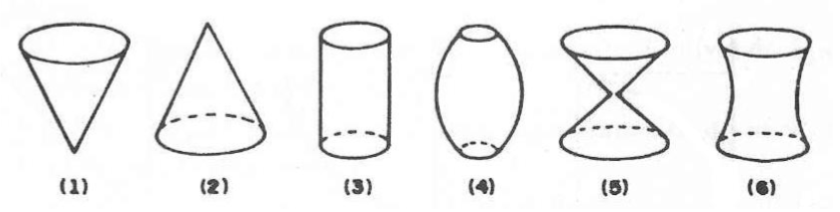
\includegraphics[width=350bp]{taxa-ativ-2-7}

% \end{figure}

\begin{multicols}{3}
\begin{enumerate}[label=(\Roman*)]
\item \begin{tikzpicture}[scale=.4,baseline=(current bounding box.north), every node/.style={scale=.8}]


\draw [->] (0,0) -- (5,0) node [below] {T};
\draw [->] (0,0) -- (0,5) node [left] {A};

\clip (0,0) rectangle (4,4);
\draw [dashed] (4,0) -- (4,4) -- (0,4);

\draw [thick] (0,0) .. controls (3,2) and (2,3) ..  (4,4);

\end{tikzpicture}

\item\begin{tikzpicture}[scale=.4,baseline=(current bounding box.north), every node/.style={scale=.8}]


\draw [->] (0,0) -- (5,0) node [below] {T};
\draw [->] (0,0) -- (0,5) node [left] {A};

\clip (0,0) rectangle (4,4);
\draw [dashed] (4,0) -- (4,4) -- (0,4);

\draw [thick] (4,0) circle (4);

\end{tikzpicture}

\item\begin{tikzpicture}[scale=.4,baseline=(current bounding box.north), every node/.style={scale=.8}]


\draw [->] (0,0) -- (5,0) node [below] {T};
\draw [->] (0,0) -- (0,5) node [left] {A};

\clip (0,0) rectangle (4,4);
\draw [dashed] (4,0) -- (4,4) -- (0,4);

\draw [thick] (0,0) .. controls (1,3) and (3,1) ..  (4,4);

\end{tikzpicture}

\item\begin{tikzpicture}[scale=.4,baseline=(current bounding box.north), every node/.style={scale=.8}]


\draw [->] (0,0) -- (5,0) node [below] {T};
\draw [->] (0,0) -- (0,5) node [left] {A};

\clip (0,0) rectangle (4,4);
\draw [dashed] (4,0) -- (4,4) -- (0,4);

\draw [thick] (0,0) .. controls (3,1) and (1,3) ..  (4,4);

\end{tikzpicture}

\item\begin{tikzpicture}[scale=.4,baseline=(current bounding box.north), every node/.style={scale=.8}]


\draw [->] (0,0) -- (5,0) node [below] {T};
\draw [->] (0,0) -- (0,5) node [left] {A};

\clip (0,0) rectangle (4,4);
\draw [dashed] (4,0) -- (4,4) -- (0,4);

\draw [thick] (0,4) circle (4);

\end{tikzpicture}

\item\begin{tikzpicture}[scale=.4,baseline=(current bounding box.north), every node/.style={scale=.8}]


\draw [->] (0,0) -- (5,0) node [below] {T};
\draw [->] (0,0) -- (0,5) node [left] {A};

\draw [dashed] (4,0) -- (4,4) -- (0,4);

\draw [thick] (0,0) -- (4,4);

\end{tikzpicture}

\end{enumerate}
\end{multicols}



\end{task}

\begin{task}{Uma viagem de carro}

Você está viajando de carro para uma cidade que está a 410 km de distância da sua casa. Você sai ao meio dia e depois de 2h de viagem faz a primeira parada em um posto de combustível na estrada. Olhando no GPS, calcula que já percorreu 140 km desde a sua partida. Depois de 30 minutos parte para a estrada novamente. Faz uma nova parada das 16h às 16h30 em outro posto 120 km adiante do anterior. E finalmente às 18h chega ao seu destino.

\begin{enumerate}
\item Preencha a tabela abaixo com as distâncias percorridas e marque no sistema de coordenadas os pares ordenados correspondentes. (o eixo horizontal representa o tempo decorrido em horas desde a partida e o eixo vertical a distância percorrida em quilômetros).

\begin{table}[H]
\centering
\begin{tabu} to \textwidth{|r|c|c|}
\hline
\thead
Horário & \parbox{3.5cm}{\centering\vspace{.5em} Tempo decorrido desde a partida (h)\vspace{.5em}} & \parbox{3.5cm}{\centering\vspace{.5em} Distância percorrida (km)\vspace{.5em}} \\
\hline
& $t$ & $d(t)$ \\
\hline
12h & 0 & \\
\hline
14h & 2 & \\
\hline
14h30 & 2.5 & \\
\hline
16h & & \\
\hline
16h30 & & \\
\hline
18h & & \\
\hline
\end{tabu}
\end{table}

\begin{figure}[H]
\centering
\begin{tikzpicture}[scale=1.2]

\draw [gray!30, step=.25] (0,0) grid (7.25,5);
\draw [gray!70] (0,0) grid (7.25,5);
\draw [->] (0,0) -- (7.25,0) node [below, shift={(0,-.5)}, pos=.82] {tempo desde a partida (h)};
\draw [->] (0,0) -- (0,5) node [pos=.75,above, rotate=90, shift={(-1,.6)}] {distância percorrida (km)};
\foreach \x in {1,...,7} \node [below] at (\x,0) {\x};
\foreach \x in {1,...,4} \node [left] at (0,\x) {\x00};
\node [below left] at (0,0) {0};

\end{tikzpicture}
\end{figure}
\item A distância total percorrida na viagem foi de 410 km, e durou 6h. Podemos obter a \textbf{velocidade média} da viagem dividindo esses dois valores, obtendo
\begin{equation*}
\frac{\Delta d}{\Delta t}=\frac{410}{6}=51,5 \cdot \frac{km}{h}
\end{equation*}
O que representa esse número no contexto do problema?
\item Calcule a velocidade média para o trecho da partida até chegar à primeira parada
\begin{equation*}
\frac{\Delta d}{\Delta t}=\cdot=\frac{km}{h}
\end{equation*}
Ele é o mesmo que o anterior? Explique
\item Sem fazer a conta, você imagina que o valor da velocidade média no trecho da partida até a hora de sída a primeira parada (14h30) será maior ou menor que o valor do item anterior? Por que?
\item preencha a tabela com as velocidade médias nostrechos indicados.

\begin{table}[H]
\centering
\setlength\tabulinesep{1mm}
\begin{tabu} to \textwidth{|c|c|}
\hline
\thead
Intervalo de tempo $a,b$ & \makecell{Velocidade média \vspace{.3em}\\  $\bm{\displaystyle \frac{\Delta d}{\Delta t} = \frac{d(b)-(d(a)}{b-a}}$} \\
\hline
$0,2$ & \\
\hline
$2,2.5$ & \\
\hline
$2.5,4$ & \\
\hline
$4,4.5$ & \\
\hline
$4.5,6$ & \\
\hline
\end{tabu}
\end{table}
\end{enumerate}

\end{task}

\clearpage
\arrange{}

A taxa de variação de uma grandeza em relação a outra é a medida do ritmo de crescimento ou decrescimento entre tais grandezas. É quanto uma grandeza varia por unidade da outra. 

Quando se diz que um recipiente está sendo enchido com um líquido à uma taxa de variação constante de $1\ell/min$ (um litro por minuto) significa que a cada minuto transcorrido, 1 litro de líquido é acrescido ao recipiente. A velocidade é a taxa de variação do espaço percorrido por unidade de tempo. Dizer que um carro tem uma velocidade uniforme de $50km/h$ significa que se mantiver essa velocidade por uma hora, percorrerá uma distância de 50 quilômetros.

Nem sempre estamos diante de situações em que as taxas de variação entre as grandezas são constantes (uniformes). Nestes casos, precisamos considerar a variação média dos valores de uma grandeza em um dado intervalo de valores da outra. Mais precisamente, considere uma $y$ grandeza  que pode ser expressa como função da grandeza $x$, isto é, $y=f(x)$. A \textbf{taxa de variação média} de $y$ em relação a $x$ no intervalo $[a,b]$ é definida por
\begin{equation*}
\frac{\Delta y}{\Delta x}=\frac{f(b)-f(a)}{a-b}
\end{equation*}
Ou seja, é a razão entre a variação total de $y=f(x)$ e o comprimento do intervalo. POr exemplo, se a temperatura ($T$) de um corpo aumenta de $36^{\circ}C$ para $39^{\circ}C$ no intervalo de tempo ($t$) entre 10h00min e 10h15min podemos dizer que a taxa de variação média da temperatura nesse intervalo de tempo é de
\begin{equation*}
\frac{\Delta T}{\Delta t}=\frac{39^{\circ}C-36^{\circ}}{10h15min-10h00min}=\frac{3^{\circ}C}{15 min}=0,2^{\circ}C/min
\end{equation*}

Isso não significa que às 10h01min a temperatura era de $36,2^{\circ}C$ às $36,4^{\circ}C$ e assim sucessivamente. Apenas pode-se dizer que \textbf{em médica}, a cada minuto, houve um aumento dessa magnitude. A taxa de variação média trata de informação apenas no início e no fim do intervalo.

O gráfico e a tabela a seguir mostram a variação do número de visualizações (\textit{views}) de um determinado vídeo no YouTube ao longo de uma semana.

\begin{minipage}{0.4\textwidth}
\centering
\begin{tabu} to \textwidth{|c|c|}
\hline
\thead
Dia ($d$) & Visualizações ($V$) \\
\hline
0&0 \\
\hline
1&12 \\
\hline
2&40 \\
\hline
3&102 \\
\hline
4&160 \\
\hline
5&250 \\
\hline
6&200 \\
\hline
7&132 \\
\hline
\end{tabu}
\end{minipage}
\begin{minipage}{0.6\textwidth}
\centering
\begin{tikzpicture}[every node/.style={scale=.8}, xscale=1.5, scale=.75]

\draw [gray!30, step=.25] (0,0) grid (7.25,6);
\draw [gray!60] (0,0) grid (7.25,6);
\draw [->] (0,0) -- (7.25,0);
\draw [->] (0,0) -- (0,6);
\foreach \x in {1,...,7} \node [below] at (\x,0) {\x};
\foreach \x/\y in {1/50,2/100,3/150,4/200,5/250} \node [left] at (0,\x) {\y};
\node [below left] at (0,0) {0};

\coordinate (a) at (0,0);
\coordinate (b) at (1,.12*2);
\coordinate (c) at (2,.4*2);
\coordinate (d) at (3,1.02*2);
\coordinate (e) at (4,1.60*2);
\coordinate (f) at (5,2.50*2);
\coordinate (g) at (6,2*2);
\coordinate (h) at (7,1.32*2);

\draw [very thick, \currentcolor!80] (a) -- (b) -- (c) -- (d) -- (e) -- (f) -- (g) -- (h);
\foreach \x in {a,...,h} \node [fill, circle, inner sep=2pt, \currentcolor!80] at (\x) {};
\end{tikzpicture}
\end{minipage}

Perceba que a taxa de variação média entre os dias 1 e 7 é a mesma observada entre os dias 4 e 6, ao mesmo tempo que os valores intermediários são bem distintos.
\begin{align*}
\frac{\Delta V}{\Delta d}=&\frac{132-12}{7-1}=\frac{120}{6}=20\:views/dia \\
\frac{\Delta V}{\Delta d}=&\frac{200-160}{6-1}=\frac{120}{6}=20\:views/dia
\end{align*}

Agora, vamos destacar um outro aspecto importante da taxa de variação. Vamos calcular, nesse último exemplo a taxa de variação média entre os dias 5 e 7:

\begin{equation*}
\frac{\Delta V}{\Delta d}=\frac{132-250}{7-5}=\frac{-118}{2}=-59\:views/dia
\end{equation*}

Por que esse resultado foi negativo? O que isso pode significar? Qual a relação dele com o aspecto do gráfico?

O resultado foi negativo pois a quantidade de visualizações no dia 7 foi menor do que a quantidade no dia 5, fazendo com que o resultado da subtração no numerador fosse negativo e indicando que houve, no período analisado, uma queda no número de visualizações. Dá para conjecturar que sempre que houver essa redução, teremos uma taxa de variação média negativa o que tem relação com algum tipo de decrescimento global da função nesse intervalo.

\begin{minipage}{0.33\textwidth}
\begin{tikzpicture} 

\draw [gray!30, step=.2] (0,0) grid (5,4);
\draw [gray!60] (0,0) grid (5,4);
\draw [thick] (0,4) -- (0,0) -- (5,0);

\draw [fill] (1,2) circle (1.5pt);
\draw [fill] (4,1) circle (1.5pt);
\draw [dashed] (1,2) -- (4,1);

\draw [thick] (1,2) .. controls (1,4) and (3,2.5) .. (4,1);


\end{tikzpicture}
\end{minipage}
\begin{minipage}{0.33\textwidth}
\begin{tikzpicture} 

\draw [gray!30, step=.2] (0,0) grid (5,4);
\draw [gray!60] (0,0) grid (5,4);
\draw [thick] (0,4) -- (0,0) -- (5,0);

\draw [fill] (1,2) circle (1.5pt);
\draw [fill] (4,1) circle (1.5pt);
\draw [dashed] (1,2) -- (4,1);

\draw [thick] (1,2) .. controls (2,0) and (2,4) .. (4,1);

\end{tikzpicture}
\end{minipage}
\begin{minipage}{0.33\textwidth}
\begin{tikzpicture} 

\draw [gray!30, step=.2] (0,0) grid (5,4);
\draw [gray!60] (0,0) grid (5,4);
\draw [thick] (0,4) -- (0,0) -- (5,0);

\draw [fill] (1,2) circle (1.5pt);
\draw [fill] (4,1) circle (1.5pt);
\draw [dashed] (1,2) -- (4,1);

\draw [thick] (1,2) .. controls (2,4) and (3,0) .. (4,1);

\end{tikzpicture}
\end{minipage}

O numerador da taxa de variação média é a diferença entre os valores final e inicial. Assim, sempre que o valor final for menor que o inicial, o numerador $\Delta y$ será negativo. Como o denominador $\Delta x$ é sempre positivo, o resultado da razão entre eles será um número negativo. 

Como mencionado antes, a taxa de variação média diz respeito apenas às imagens dos extremos do intervalo. Portanto, ao observarmos que em um determinado intervalo a taxa média foi negativa, não podemos afirmar que a função é decrescente em todo intervalo, mas apenas que houve mais decrescimento do que crescimento, em média. Os três gráficos acima têm taxa média negativa no intervalo destacado.

Com um raciocínio similar, podemos dizer que uma taxa de variação média positiva indica um crescimento entre os valores inicial e final da variável dependente no intervalo considerado, mas não que a função é crescente em todo o intervalo.

\begin{minipage}{0.5\textwidth}
\begin{tikzpicture}

\draw [gray!30, step=.2] (-3,-2) grid (5,3);
\draw [gray!60] (-3,-2) grid (5,3);
\draw [thick] (0,3) -- (0,-2);
\draw [thick] (-3,0) -- (5,0);

\draw [fill] (-2,-1) circle (1.5pt);
\draw [fill] (4,1) circle (1.5pt);
\draw [dashed] (-2,-1) -- (4,1);

\draw [thick] (-2,-1) .. controls (-2,3) and (3,-2) .. (4,1);

\end{tikzpicture}
\end{minipage}
\begin{minipage}{0.5\textwidth}
\begin{tikzpicture} 

\draw [gray!30, step=.2] (-3,-2) grid (5,3);
\draw [gray!60] (-3,-2) grid (5,3);
\draw [thick] (0,3) -- (0,-2);
\draw [thick] (-3,0) -- (5,0);

\draw [fill] (-2,-1) circle (1.5pt);
\draw [fill] (4,1) circle (1.5pt);
\draw [dashed] (-2,-1) -- (4,1);

\draw [thick] (-2,-1) .. controls (0,-2) and (2,2) .. (4,1);

\end{tikzpicture}
\end{minipage}

\begin{figure}[H]
\centering
\begin{tikzpicture} 

\draw [gray!30, step=.2] (-3,-2) grid (5,3);
\draw [gray!60] (-3,-2) grid (5,3);
\draw [thick] (0,3) -- (0,-2);
\draw [thick] (-3,0) -- (5,0);

\draw [fill] (-2,-1) circle (1.5pt);
\draw [fill] (4,1) circle (1.5pt);
\draw [dashed] (-2,-1) -- (4,1);

\draw [thick] (-2,-1) .. controls (1,-0) and (3.5,-2) .. (4,1);

\end{tikzpicture}
\end{figure}

\textbf{Lentamente, uniformemente ou rapidamente?}

\begin{wrapfigure}[13]{r}{0.5\textwidth}
\centering
\vspace{-1em}
\begin{tikzpicture}[scale=1]
\draw [gray!30, step=.2] (-1,-1) grid (7,5);
\draw [gray!60] (-1,-1) grid (7,5);
\draw [thick] (0,-1) -- (0,5);
\draw [thick] (-1,0) -- (7,0);
\draw [fill] (0,1) circle (1.5pt);
\draw [fill] (2,2) circle (1.5pt);
\draw [fill] (4,3) circle (1.5pt);
\draw [fill] (6,4) circle (1.5pt);
\draw [dashed, thick] (0,1) -- (2,1)node [below, pos=.5] {$\Delta x$} -- (2,2) node [right, midway] {$\Delta y$};
\draw [dashed, thick] (4,3) -- (6,3) node [below, pos=.5] {$\Delta x$} -- (6,4) node [right, midway] {$\Delta y$};
\draw [thick, domain=-1:7] plot (\x,1/2*\x+1);
\foreach \x/\y in {.95/1,1.05/1,4.95/3,5.05/3} \draw [thick] (\x,\y+.1) -- (\x,\y-.1);
\foreach \x/\y in {1.45/2,1.5/2,1.55/2,3.45/6,3.5/6,3.55/6} \draw [thick] (\y+.1,\x) -- (\y-.1,\x);
\end{tikzpicture}
\end{wrapfigure}
Os adjetivos acima somente fazem sentido quando estamos comparando o crescimento de duas ou mais funções ou a mesma função em dois ou mais intervalos diferentes. 

Por exemplo, dizer que uma determinada função \textbf{cresce uniformemente} significa que para intervalos $\Delta x$ iguais a variável $y$ apresentou a mesma variação, isto é, se dois intervalos do domínio têm o mesmo $\Delta x$, correspondendo a eles teremos o mesmo $\Delta y$. Em termos da taxa de variação podemos dizer que ambos os intervalos apresentam a mesma taxa média. Na verdade, só poderemos afirmar que há algum tipo de uniformidade se isso acontecer para quaisquer dois intervalos! Veja a figura ao lado. Esse caso será tratado com maiores detalhes no capítulo sobre as funções afins.\par

Nos casos em que a taxa média não é sempre a mesma, podemos comparar dois intervalos com taxas médias positivas distintas e dizer que onde a taxa for menor a função cresceu em média mais lentamente do que no outro intervalo onde a taxa média foi maior. Para o caso da taxa média negativa, acontece o oposto: quanto menor for o valor, mais decrescimento houve no intervalo.

Nos gráficos a seguir, os comprimentos dos intervalos $\Delta x$ são iguais, mas os comprimentos dos respectivos $\Delta y$ variam.

\begin{figure}[H]
\centering
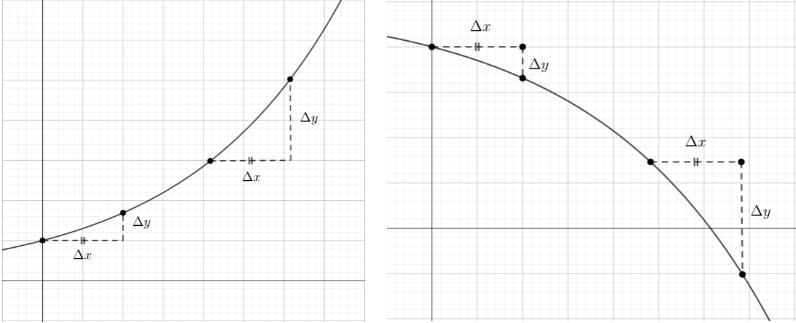
\includegraphics[width=300bp]{taxa-arrange-8}
\end{figure}

\clearpage
\def\currentcolor{session2}
\begin{objectives}{Hora de encher a piscina}
{
\begin{itemize}

\item Utilizar o vocabulário associado ao conceito de taxa de variação para descrever com palavras uma situação real (item a).

\item Associar uma situação real a uma representação gráfica (item b).

\item Diferenciar situações de crescimento, identificando quando o gráfico pode ser uma linha reta – taxa de variação constante (item a) e quando não (item b).

\end{itemize}
}{1}{2}
\end{objectives}
\begin{sugestions}{Hora de encher a piscina}
{
\begin{itemize}
\item É importante que o estudante perceba que no item a), tanto na primeira parte do
enchimento quanto na segunda parte, a profundidade $d$ aumenta uniformemente. É
desejável que eles se expressem utilizando expressões como “$d$ aumenta
uniformemente”.
\item Ainda no item a), é esperado que o estudante perceba que há uma mudança na taxa em
que $d$ aumenta. Isto é, na primeira parte do enchimento da piscina a profundidade $d$
aumenta mais rapidamente do que na segunda parte do enchimento.
\item Para o item b) há algumas possibilidades de gráficos que representam corretamente a
situação. É importante observar se os estudantes perceberam que o gráfico começa em
$(0,0)$, termina em $(30,2)$ e apresenta uma mudança em $(x, 1)$, com $5\leq x \leq 10$, por
exemplo.
\item Após a realização da atividade discuta com os estudantes sobre a justificativa para o
gráfico que representa a primeira parte do enchimento no item b) ser curvo com
concavidade voltada para baixo.
\end{itemize}
}{1}{2}
\end{sugestions}
\begin{answer}{Hora de encher a piscina}
{
\begin{enumerate}
\item A profundidade de $d$, da água até o fundo da piscina, aumenta uniformemente na primeira parte do enchimento. Após o enchimento dessa parte mais estreita há uma mudança na taxa com que $d$ aumenta, nesse segundo momento $d$ aumentará mais lentamente, porém esse aumento também ocorrerá de forma uniforme.

\item Um gráfico possível é:

\begin{tikzpicture}[scale=2.5, every node/.style={black},every path/.style={black}]
\draw [gray!60] (0,0) grid (3.3,3.3);
\draw [->] (0,0) -- (3.3,0) node [below left, shift={(0,-.5)}] {Tempo (minutos)};
\draw [->] (0,0) -- (0,3.3) node [above left, shift={(-.5,0)}, rotate=90] {Profundidade da água (metros)};
\foreach \x in {1,2,3}{
  \node [below] at (\x,0) {\x0};
  \node [left] at (0,\x) {\x};
};
\node [below left] at (0,0) {0};
\draw [session1, thick] (1,1) -- (3,2);
\fill (3,2) circle (1pt);
\draw [\tikzcolor, domain=0:1, thick] plot (\x,{-(\x)^2+2*\x});
\end{tikzpicture}
\end{enumerate}
}{0}
\end{answer}
\clearmargin
\begin{objectives}{Aumento da população}
{
\begin{itemize}

\item Perceber a importância do intervalo no cálculo da taxa de variação média.

\item Diferenciar “variação da função” de “taxa de variação média”.

\end{itemize}
}{1}{1}
\end{objectives}
\begin{sugestions}{Aumento da população}
{
\begin{itemize}
\item Podemos cair no equívoco de achar que a taxa de variação média total é a média
aritmética das taxas intermediárias. Nesse caso, achar que $1{,}67$ deveria ser a média
aritmética entre $2$ e $1{,}43$. Contudo, um cálculo simples mostra que não é o caso. Isso se
deve ao fato de estarmos considerando intervalos diferentes de tempo. Para funcionar
devemos fazer a média aritmética ponderada, nesse caso.
\end{itemize}
}{1}{1}
\end{sugestions}
\begin{answer}{Aumento da população}
{
\begin{enumerate}
\item Aumento de 10 milhões de pessoas. Idem.
\item Entre 2007 e 2012, pois foi um intervalo menor de tempo (5 anos) comparado aos 7 anos entre 2012 e 2019.
\item 2 milhões de pessoas a mais por ano entre 2007 e 2012. Aproximadamente 1,42 milhão de pessoas a mais por ano entre 2012 e 2019. No período total, tivemos aumento de aproximadamente $1{,}67$ milhão de pessoas por ano.
\end{enumerate}
}{0}
\end{answer}
\begin{objectives}{Gráficos, tabelas e fórmulas}
{
\begin{itemize}

\item Associar uma situação real a uma representação gráfica.

\item Registrar com palavras o comportamento observado no gráfico.

\item Construir tabelas a partir de informações dadas por uma situação.

\item Confrontar o gráfico esboçado com a tabela construída.

\end{itemize}
}{1}{1}
\end{objectives}
\begin{sugestions}{Gráficos, tabelas e fórmulas}
{
\begin{itemize}

\item Essa é uma atividade que inverte completamente a sequência tradicional fórmula $\rightarrow$
tabela $\rightarrow$ gráfico.
\item Esperamos que essa atividade forneça uma sensação “qualitativa” da natureza das
funções.

\item Para a primeira situação descrita é possível que alguns estudantes apresentem um
gráfico como o seguinte:

\begin{figure}[H]
\centering
\begin{tikzpicture}[xscale=.75, scale=.7]

\draw [->] (0,0) -- (16,0) node [below left, yshift=-.25cm] {Tempo (meses)};
\draw [->] (0,0) -- (0,9) node [above left, xshift=-.75cm, rotate=90] {Custo (reais)};
\draw [help lines] (0,0) grid (16,9);

\foreach \x in {80,160,...,800} \node [left] at (0,\x*0.01) {\x};
\foreach \x in {5,10,15} \node [below] at (\x,0) {\x};

\clip (0,0) rectangle (15,9);
\draw[domain=1:13, thick, \tikzcolor] plot (\x,{0.8*\x-0.8});
\end{tikzpicture}
\end{figure}

Caso apareça uma solução como esta, sugerimos encaminhar as discussões destacando
os seguintes fatos: o domínio a ser considerado é um conjunto discreto; o gráfico acima
representa uma situação em que considera-se o custo sendo acumulado mês a mês.

\item Encontrar uma fórmula será o principal obstáculo. Neste ponto pode ajudar bastante se
primeiro for solicitado aos estudantes que falem e depois registrem por escrito o
método que eles usaram para construir as tabelas de valores. A observação de
tendências e padrões a partir das tabelas deverá facilitar a obtenção das expressões
algébricas.

\item Os estudantes podem ter um pouco mais de dificuldade para responder ao item (d). Isso
não é grave nesse momento, e de certa forma, contribui para o entendimento que nem
sempre precisamos (ou conseguiremos) encontrar uma expressão matemática que
relacione as grandezas, mas mesmo assim podemos ter ideias qualitativas sobre o
comportamento e as variações.

\end{itemize}
}{0}{1}
\end{sugestions}
\begin{answer}{Gráficos, tabelas e fórmulas}
{
\begin{enumerate}
\item \textbf{TV por assinatura}

\begin{tikzpicture}[every node/.style={black}, every path/.style={black},scale=.5]
\draw [->] (-.5,0) -- (12,0) node [below left, yshift=-.5cm] {Tempo (meses)};
\draw [->] (0,-.5) -- (0,9) node [above left,rotate=90, yshift=1cm] {Custo da mensalidade (R\$)};
\draw [help lines] (0,0) grid (12,9);
\foreach \x in {1,...,11} \node [below] at (\x,0) {\x};
\node [left] at (0,8) {80};
\node [left] at (0,4) {40};
\node [below left] at (0,0) {0};

\fill [\tikzcolor] (1,0) circle (3pt);
\foreach \x in {2,...,10} \fill [\tikzcolor] (\x,8) circle (3pt);
\end{tikzpicture}


\textbf{Valor de mercado de um carro}


\begin{tikzpicture}[every node/.style={black}, every path/.style={black},scale=.5]
\draw [->] (-.5,0) -- (16,0) node [below left, yshift=-.5cm] {Tempo (anos)};
\draw [->] (0,-.5) -- (0,8) node [above left,rotate=90, yshift=1.5cm] {Valor do carro (R\$)};
\draw [help lines] (0,0) grid (16,8);
\foreach \x in {1,...,16} \node [below] at (\x,0) {\x};
\node [left] at (0,5) {50.000};
\node [left] at (0,2.5) {25.000};
\node [left] at (0,7.5) {75.000};
\node [below left] at (0,0) {0};

\foreach \x/\y in {0/6.5,1/6.5*.8,2/6.5*.8^2,3/6.5*.8^3,4/6.5*.8^4,5/6.5*.8^5,6/6.5*.8^6,7/6.5*.8^7,8/6.5*.8^8,9/6.5*.8^9,10/6.5*.8^10,11/6.5*.8^11,12/6.5*.8^12,13/6.5*.8^13,14/6.5*.8^14,15/6.5*.8^15} \fill [\tikzcolor] (\x,\y) circle (3pt);

\draw [domain=0:15, \tikzcolor, dashed] plot (\x,{6.5*0.8^\x});
\end{tikzpicture}

\columnbreak
\textbf{Subindo uma escada}


\begin{tikzpicture}[every node/.style={black}, every path/.style={black},scale=.7]
\draw [->] (-.5,0) -- (15,0) node [below left, yshift=-.5cm] {Altura do degrau (cm)};
\draw [->] (0,-.5) -- (0,6) node [above left,rotate=90, yshift=1cm] {Passada (cm)};
\draw [help lines] (0,0) grid (15,6);
\foreach \x/\y in {2/5,4/10,6/15,8/30,10/20,12/25,14/30} \node [below] at (\x,0) {\y};
\foreach \x/\y in {1/20,2/40,3/60,4/80,5/100} \node [left] at (0,\x) {\y};

\draw [thick, \tikzcolor] (0,3) -- (14,0);
\fill [\tikzcolor] (0,3) circle (3pt);

\node [below left] at (0,0) {0};


\end{tikzpicture}


\textbf{Polígonos regulares}


\begin{tikzpicture}[every node/.style={black}, every path/.style={black},scale=.7,yscale=.5]
\draw [->] (-.5,0) -- (14,0) node [below left, yshift=-.5cm] {Número de lados};
\draw [->] (0,-.5) -- (0,17) node [above left,rotate=90, yshift=1cm] {Tamanho de cada ângulo (graus)};
\draw [help lines] (0,0) grid (14,16);
\foreach \x in {2,4,...,14} \node [below] at (\x,0) {\x};
\foreach \x in {4,8,12,16} \node [left] at (0,\x) {\x0};

\foreach \x/\y in {3/6,4/9,5/10.8,6/12,7/12.86,8/13.5,9/14,10/14.4,11/14.727} \node [fill,circle, inner sep=1.5pt, \tikzcolor] at (\x,\y) {};

\node [below left] at (0,0) {0};
\draw [dashed, \tikzcolor, domain=3:11] plot (\x,{18-36/\x});


\end{tikzpicture}


\item \textbf{TV por assinatura} - No primeiro mês o custo é zero, nos meses seguintes é cobrado o valor fixo de R\$ 80,00, por isso o gráfico é um conjunto de pontos distribuídos sobre uma reta que intercepta o eixo $y$ no ponto $(0,80)$.

\textbf{Valor de mercado de um carro} - A cada ano o valor de mercado do automóvel vai diminuindo, no entando, a desvalorização sofrida no ano anterior será sempre maior do que a desvalorização observada no ano seguinte. Dessa forma, o gráfico terá a forma de uma curva suave que se inicia no ponto $(0,65.000) $ e se aproxima de zero na medida em que o tempo em anos aumenta.

\textbf{Subindo uma escada} - Temos uma diminuição uniforme de $2$ cm no comprimento da passada cada vez que aumentamos $1$ cm a altura do degrau. Dessa forma o gráfico será uma reta com ponto inicial em $(0,60)$ e ponto final $(30,0)$, uma vez que para um degrau de $30$ cm de altura será de $0$ cm.

\textbf{Polígonos regulares} - A medida do ângulo interno de um pólígono regular aumenta à medida em que aumentamos o número de lados. Esse aumento, no entanto, não é uniforme, uma vez que para cada lado a mais considerado o aumento corresponde percebido no ângulo interno é cada vez menor. Dessa forma o ângulo interno cresce lentamente conforme o número de lados do polígono regular aumenta.

\newpage
\item \textbf{TV por assinatura}


\begin{tabu} to \textwidth{|c|c|}
\hline
\thead
Tempo (meses) & Custo da assinatura (R\$) \\
\hline
1 & 0 \\
\hline
2 & 80 \\
\hline
3 & 80 \\
\hline
2 & 80 \\
\hline
$\vdots$ & $\vdots$ \\
\hline
\end{tabu}


\textbf{Valor de mercado de um carro}


\begin{tabu} to \textwidth{|c|c|}
\hline
\thead
Tempo (anos) & Valor de mercado do carro (R\$) \\
0 & 65.000,00 \\
\hline
1 & 52.000,00 \\
\hline
2 & 41.600,00 \\
\hline
3 & 33.280,00 \\
\hline
$\vdots$ & $\vdots$ \\
\hline
\end{tabu}
\vspace{1em}

\textbf{Subindo uma escada}


\begin{tabu} to \textwidth{|c|c|}
\hline
\thead
Altura do degrau (cm) & Comprimento da passada (cm) \\
0 & 60 \\
\hline
1 & 58 \\
\hline
2 & 56 \\
\hline
3 & 54 \\
\hline
$\vdots$ & $\vdots$ \\
\hline
\end{tabu}

\vspace{1em}
\textbf{Polígonos regulares}


\begin{tabu} to \textwidth{|c|c|}
\hline
\thead
Número de lados & Tamanho de cada ângulo (graus) \\
3 & 60 \\
\hline
4 & 90 \\
\hline
5 & 108 \\
\hline
6 & 120 \\
\hline
7 & 128,6 \\
\hline
8 & 135 \\
\hline
$\vdots$ & $\vdots$ \\
\hline
\end{tabu}


\item \textbf{TV por assinatura}

\[C(t)
\begin{cases}
0,\text{ se } t=1\\
80,\text{ se } t=2,3,4,...
\end{cases}
\]
\begin{center}
$C$ - valor fixo da mensalidade em reais, $t$=período de assinatura em meses.
\end{center}

\clearpage
\textbf{Valor de mercado de um carro}
\begin{equation*}
V(t)=65.000\times 0,8^t
\end{equation*}
\begin{center}
$V$ = valor do carro em reais, $t$= idade do carro em anos.
\end{center}

\textbf{Subindo uma escada}
\begin{equation*}
P(h)=60-2h
\end{equation*}
\begin{center}
$P$ = medida passada em centímetros, $h$=altura do degrau em centímetros.
\end{center}

\textbf{Polígonos regulares}
\begin{equation*}
A(n)=180-\frac{360}{n}
\end{equation*}
\begin{center}
$A$=medida de cada ângulo interno, $n$=número de lados do polígono regular.
\end{center}
\end{enumerate}
}{9}
\end{answer}
\clearmargin
\begin{objectives}{As imagens}
{
\begin{itemize}

\item  Calcular imagens de alguns pontos sendo conhecidas as taxas de variação médias em intervalos do domínio.

\item Relacionar a disposição dos pontos no gráfico com a variação da taxa de variação média.

\end{itemize}
}{1}{2}
\end{objectives}
\marginpar{\vspace{-2em}}
\begin{sugestions}{As imagens}
{
\begin{itemize}

\item A principal atenção na hora de fazer as contas deve estar nos intervalos em que estão
definidas as taxas médias.
\item Ao finalizar a atividade, estimule que os estudantes façam conjecturas sobre a variação
da taxa e a forma do gráfico. Por exemplo, “o que ocorre quando a taxa é igual a zero?”,
“se for constante e positiva?”, “constante e negativa?”, “qual a forma do gráfico quando
a taxa de variação é crescente?", “e decrescente?” etc.
\item Como extensão, proponha que os estudantes investiguem que taxas médias gerariam
outras formas de gráficos; desafie-os a conjecturar ou pelo menos a dar exemplos de
taxas que correspondam às formas abaixo,

\begin{multicols}{5}
\begin{center}

\begin{tikzpicture}

\draw (-1,0) -- (1,0);
\draw (0,-1) -- (0,1);

\draw [domain=-1:1, \tikzcolor, thick] plot (\x,{\x^3});
\end{tikzpicture}

\begin{tikzpicture}

\draw (-1,0) -- (1,0);
\draw (0,-1) -- (0,1);

\draw [domain=-1:1, \tikzcolor, thick] plot (\x,{-\x^3});
\end{tikzpicture}

\begin{tikzpicture}

\draw (-1,0) -- (1,0);
\draw (0,-1) -- (0,1);

\draw [domain=-1:1, \tikzcolor, thick] plot (\x,{-(\x)^2});
\end{tikzpicture}

\begin{tikzpicture}

\draw (-1,0) -- (1,0);
\draw (0,-1) -- (0,1);

\draw [domain=-1:1, \tikzcolor, thick] plot (\x,{(\x)^2});
\end{tikzpicture}

\begin{tikzpicture}

\draw (-1,0) -- (1,0);
\draw (0,-1) -- (0,1);

\draw [domain=0:1, \tikzcolor, thick] plot (\x,{(\x)^2-2*(\x)});

\draw [domain=0:-1, \tikzcolor, thick] plot (\x,{-(\x)^2-2*(\x)});

\end{tikzpicture}

\end{center}
\end{multicols}
\end{itemize}
}{1}{0}
\end{sugestions}
\begin{answer}{As imagens}
{
\begin{enumerate}

\tikzstyle{circ}=[fill,circle, inner sep=1.5pt, \tikzcolor]
\item\adjustbox{valign=t}{
\begin{tikzpicture}[yscale=.5,xscale=1.2, every node/.style={black}, every path/.style={black}]
    \draw [->, thick] (0,-.5) -- (0,11) node[left] {$y$};
    \draw [->, thick] (-.5,0) -- (4.2,0) node[below] {$x$};
    \draw[help lines, gray] (0,0) grid (4.01,10.01);
    \foreach \x in {1,...,4} \draw (\x,.1)  -- (\x,-.1)  node[below] {\x};
    \foreach \y in {1,...,10} \draw (.1,\y) -- (-.1,\y) node[left] {\y};        
\node[below left] at (0,0) {0};
\draw [dashed,\tikzcolor, thick] (0,1) -- (4,9);
\foreach \x/\y in {0/1,1/3,2/5,3/7,4/9} \node [circ] at (\x,\y) {};
  \end{tikzpicture}}
\end{enumerate}
}{1}
\end{answer}
\clearmargin
\marginpar{\vspace{.5em}}
\begin{answer}{As imagens}
{
\begin{enumerate}\setcounter{enumi}{1}
\tikzstyle{circ}=[fill,circle, inner sep=1.5pt, \tikzcolor]
\item\adjustbox{valign=t}{
\begin{tikzpicture}[yscale=.5,xscale=1.2, every node/.style={black}, every path/.style={black}]
    \draw [->, thick] (0,-.5) -- (0,11) node[left] {$y$};
    \draw [->, thick] (-.5,0) -- (4.2,0) node[below] {$x$};
    \draw[help lines, gray] (0,0) grid (4.01,10.01);
    \foreach \x in {1,...,4} \draw (\x,.1)  -- (\x,-.1)  node[below] {\x};
    \foreach \y in {1,...,10} \draw (.1,\y) -- (-.1,\y) node[left] {\y};        
\node[below left] at (0,0) {0};
\draw [dashed,\tikzcolor, thick] (0,10) -- (4,2);
\foreach \x/\y in {0/10,.5/9,1/8,1.5/7,2/6,2.5/5,3/4,3.5/3,4/2} \node [circ] at (\x,\y) {};
  \end{tikzpicture}}

\item\adjustbox{valign=t}{
\begin{tikzpicture}[yscale=.25,xscale=.6, every node/.style={black}, every path/.style={black}]
    \draw [->, thick] (0,-.5) -- (0,22) node[left] {$y$};
    \draw [->, thick] (-.5,0) -- (8.7,0) node[below] {$x$};
    \draw[help lines, gray] (0,0) grid (8.01,21);
    \foreach \x in {1,...,8} \draw (\x,.1)  -- (\x,-.1)  node[below] {\x};
    \foreach \y in {5,10,...,20} \draw (.1,\y) -- (-.1,\y) node[left] {\y};        
\node[below left] at (0,0) {0};
\draw [dashed,\tikzcolor, thick] (0,0) -- (2,2) -- (4,6) -- (6,12) -- (8,20);
\foreach \x/\y in {0/0,2/2,4/6,6/12,8/20} \node [circ] at (\x,\y) {};
  \end{tikzpicture}}

\item\adjustbox{valign=t}{
\begin{tikzpicture}[yscale=.5,xscale=1.2, every node/.style={black}, every path/.style={black}]
    \draw [->, thick] (0,-.5) -- (0,11) node[left] {$y$};
    \draw [->, thick] (-.5,0) -- (4.2,0) node[below] {$x$};
    \draw[help lines, gray] (0,0) grid (4.01,10.01);
    \foreach \x in {1,...,4} \draw (\x,.1)  -- (\x,-.1)  node[below] {\x};
    \foreach \y in {1,...,10} \draw (.1,\y) -- (-.1,\y) node[left] {\y};        
\node[below left] at (0,0) {0};
\draw [dashed,\tikzcolor, thick] (0,0) -- (1,10) -- (2,2) -- (3,8) -- (4,8);
\foreach \x/\y in {0/0,1/10,2/2,3/8,4/8} \node [circ] at (\x,\y) {};
  \end{tikzpicture}}
\end{enumerate}
}{1}
\end{answer}
\clearmargin
\marginpar{\vspace{.5em}}
\begin{answer}{As imagens}
{
\begin{enumerate}\setcounter{enumi}{4}
\tikzstyle{circ}=[fill,circle, inner sep=1.5pt, \tikzcolor]
\item\adjustbox{valign=t}{
\begin{tikzpicture}[yscale=.25,xscale=.6, every node/.style={black}, every path/.style={black}]
    \draw [->, thick] (0,-.5) -- (0,27) node[left] {$y$};
    \draw [->, thick] (-.5,0) -- (8.7,0) node[below] {$x$};
    \draw[help lines, gray] (0,0) grid (8.01,25.01);
    \foreach \x in {1,...,8} \draw (\x,.1)  -- (\x,-.1)  node[below] {\x};
    \foreach \y in {5,10,...,25} \draw (.1,\y) -- (-.1,\y) node[left] {\y};        
\node[below left] at (0,0) {0};
\draw [dashed,\tikzcolor, thick] (0,0) -- (1,1) -- (2,4) -- (3,8) -- (4,15) -- (5,20) -- (6,23) -- (7,24) -- (8,24);
\foreach \x/\y in {0/0,1/1,2/4,3/8,4/15,5/20,6/23,7/24,8/24} \node [circ] at (\x,\y) {};
  \end{tikzpicture}}
\end{enumerate}
}{1}
\end{answer}


\practice{}

\begin{task}{hora de encher a piscina}
Uma piscina retangular está sendo cheia com uma mangueira que fornece água a uma taxa constante. Uma seção transversal da piscina é mostrada na imagem a seguir.

\begin{figure}[H]
\centering
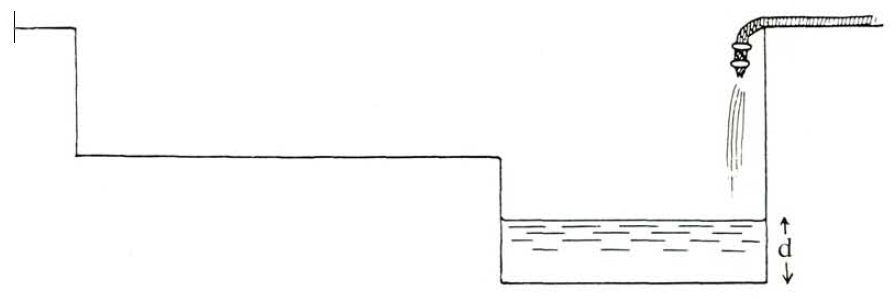
\includegraphics[width=300bp]{taxa-ativ-3-1}
\end{figure}

\begin{enumerate}
\item Descreva em palavras como a profundidade $d$ da água até o fundo da piscina varia com o tempo, a partir do momento em que a piscina vazia começa a encher.
\item Uma piscina retangular está sendo cheia de maneira semelhante.

\begin{figure}[H]
\centering
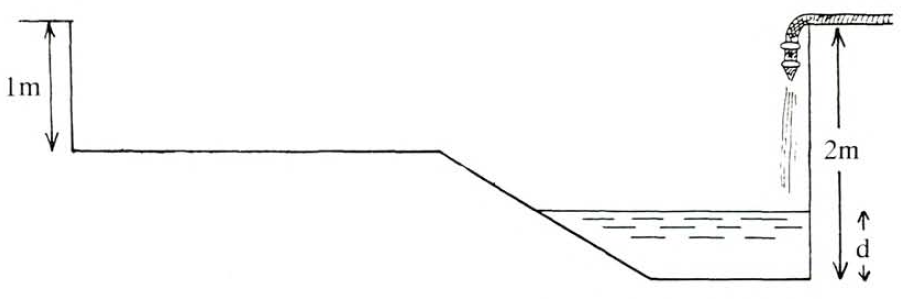
\includegraphics[width=300bp]{taxa-ativ-3-2}

\end{figure}

Supondo que a piscina leva 30 minutos para encher até a borda. Esboce um gráfico para mostrar como a profundidade $d$ da água até o fundo da piscina varia com o tempo a partir do momento em que a piscina está vazia.

\begin{figure}[H]
\centering

\begin{tikzpicture}[scale=1.5]
\draw [gray!60] (0,0) grid (3.3,3.3);
\draw [->] (0,0) -- (3.3,0) node [below left, shift={(0,-.5)}] {Tempo (minutos)};
\draw [->] (0,0) -- (0,3.3) node [above left, shift={(-.5,0)}, rotate=90] {Profundidade da água (metros)};
\foreach \x in {1,2,3}{
	\node [below] at (\x,0) {\x0};
	\node [left] at (0,\x) {\x};
};
\node [below left] at (0,0) {0};
\end{tikzpicture}
\end{figure}
\end{enumerate}
\end{task}

\begin{task}{Aumento da população}
A população brasileira alcançou os 210,1 milhões de habitantes em 2019. Segundo dados do IBGE houve um aumento de 0,79\% em relação a 2018 quando o instituto estimou a população do país em 208,5 milhões de habitantes. A tabela abaixo mostra a população aproximada de brasileiros nos anos de 2007, 2012 e 2019.

\begin{table}[H]
\centering
\begin{tabu} to \textwidth{|c|c|}
\hline
\thead
População aproximada & Ano \\
\hline
190 milhões & 2007 \\
\hline
200 milhões & 2012 \\
\hline
210 milhões & 2019 \\
\hline
\end{tabu}
\end{table}
\begin{enumerate}
\item Qual foi a variação da população entre 2007 e 2012? E entre 2012 e 2019?
\item Quando a população aumentou mais rápido? Explique.
\item De quanto foi o aumento médio anual entre 2007 e 2012? E entre 2012 e 2019? E entre 2007 e 2019?
\end{enumerate}
\end{task}

\begin{task}{Gráficos, tabelas e fórmulas}
Para cada uma das situações a seguir:
\begin{enumerate}
\item Responda à pergunta fazendo o esboço de um gráfico
\item Descreva com palavras a forma do seu gráfico
\item Verifique seu gráfico construindo uma tabela de valores. Caso seja necessário, refaça seu esboço
\item Tente encontrar uma expressão algébrica que descreva a situação
\end{enumerate}

\begin{description}\item[TV por assinatura]
Uma empresa de TV por assinatura cobra R\$ 80,00 por mês por um determinado pacote de canais. Uma oferta para novos assinantes oferece o primeiro mês gratuitamente. Como irá variar o custo da assinatura conforme o período de tempo aumenta?
\item[Valor de mercado de um carro]
Comprei um carro por R\$ 65.000,00 e seu valor está depreciando a uma taxa de 20\% ao ano. Isso significa que depois de um ano seu valor era de $60.000\times 0,8=52.000$, depois de dois anos, $52.000\times 0,8=41.600$ e assim por diante. Como o valor de mercado desse carro continuará a mudar?
\item[Subindo uma escada]
Uma passada normal tem em média 60cm de compreimento. Ela deve diminuir 2cm para cada 1cm que o pé é levantado quando estamos subindo os degraus de uma escada. Seguindo esse princípio, como deve varia o comprimento da passada com a altura de um degrau?
\item[Polígonos Regulares]
Como a medida de um dos ângulos internos depende do número de lados de um polígono regular?
\end{description}

\setlength{\columnsep}{0pt}
\begin{multicols}{8}

\begin{tikzpicture}[scale=.7*1.333]

% \draw circle (1.333*0.5cm);
\foreach \x/\y in {a/90:1,b/210:1,c/330:1}
 \coordinate (\x) at (\y);

\clip[draw] (a) -- (b) -- (c) -- cycle;
\draw (b) circle (6pt);
\end{tikzpicture} 

\begin{tikzpicture}[scale=.7*sqrt(2)]
% \draw circle (1.414213562*0.5cm);
\foreach \x/\y in {a/45:1,b/135:1,c/225:1,d/315:1} \coordinate (\x) at (\y);


\clip[draw] (a) -- (b) -- (c) -- (d) -- cycle;
\draw (225:1) circle (6pt);

\end{tikzpicture} 

\begin{tikzpicture}[scale=.7*1.1056]
% \draw circle (1cm);
\foreach \x/\y in {a/90:1,b/90+72:1,c/90+72*2:1,d/90+72*3:1,e/90+72*4:1} \coordinate (\x) at (\y);


\clip[draw] (a) -- (b) -- (c) -- (d) -- (e) -- cycle;
\draw (90+72*2:1) circle (6pt);


\end{tikzpicture} 

\begin{tikzpicture}[scale=.7*1.155]
% \draw circle (1cm);
\foreach \x/\y in {a/0:1,b/60:1,c/60*2:1,d/60*3:1,e/60*4:1,f/60*5:1} \coordinate (\x) at (\y);


\clip[draw] (a) -- (b) -- (c) -- (d) -- (e) -- (f) -- cycle;
\draw (60*4:1) circle (6pt);


\end{tikzpicture} 

\begin{tikzpicture}[scale=.7*1.052]
% \draw circle (1cm);
\foreach \x/\y in {a/90:1,b/90+51.428571429:1,c/90+51.428571429*2:1,d/90+51.428571429*3:1,e/90+51.428571429*4:1,f/90+51.428571429*5:1, g/90+51.428571429*6:1} \coordinate (\x) at (\y);


\clip[draw] (a) -- (b) -- (c) -- (d) -- (e) -- (f) -- (g) -- cycle;
\draw (90+51.428571429*3:1) circle (6pt);


\end{tikzpicture} 

\begin{tikzpicture}[scale=.7*1.082]
% \draw circle (1cm);
\foreach \x/\y in {a/22.5:1,b/22.5+45*1:1,c/22.5+45*2:1,d/22.5+45*3:1,e/22.5+45*4:1,f/22.5+45*5:1, g/22.5+45*6:1,h/22.5+45*7:1} \coordinate (\x) at (\y);


\clip[draw] (a) -- (b) -- (c) -- (d) -- (e) -- (f) -- (g) -- (h) -- cycle;
\draw (22.5+45*5:1) circle (6pt);


\end{tikzpicture} 

\begin{tikzpicture}[scale=.7*1.031]
% \draw circle (1cm);
\foreach \x/\y in {a/90:1,b/90+40*1:1,c/90+40*2:1,d/90+40*3:1,e/90+40*4:1,f/90+40*5:1, g/90+40*6:1,h/90+40*7:1,i/90+40*8:1} \coordinate (\x) at (\y);


\clip[draw] (a) -- (b) -- (c) -- (d) -- (e) -- (f) -- (g) -- (h) -- (i) -- cycle;
\draw (e) circle (6pt);



\end{tikzpicture} 

\begin{tikzpicture}[scale=.7*1.051]
% \draw circle (1cm);
\foreach \x/\y in {a/0:1,b/36*1:1,c/36*2:1,d/36*3:1,e/36*4:1,f/36*5:1, g/36*6:1,h/36*7:1,i/36*8:1,j/36*9:1} \coordinate (\x) at (\y);


\clip[draw] (a) -- (b) -- (c) -- (d) -- (e) -- (f) -- (g) -- (h) -- (i) -- (j) -- cycle;
\draw (h) circle (6pt);


\end{tikzpicture} 

\end{multicols}


\textbf{Sugestão:} Você pode calcular a soma de todos os ângulos internos de cada um dos polígonos subdividindo-os em triângulos, por exemplo: 

% \begin{center}
% 
% \end{center}

\begin{minipage}{0.5\textwidth}
\centering
\begin{tikzpicture}[scale=1.5]
\foreach \x/\y in {a/0:1,b/60:1,c/60*2:1,d/60*3:1,e/60*4:1,f/60*5:1} \coordinate (\x) at (\y);


\clip[draw] (a) -- (b) -- (c) -- (d) -- (e) -- (f) -- cycle;

\draw (e) -- (a);
\draw (e) -- (b);
\draw (e) -- (c);

\end{tikzpicture}
\end{minipage}
\begin{minipage}{0.5\textwidth}
Soma dos ângulos internos: $4\times180^{\circ}=720^{\circ}$
\end{minipage}

\end{task}

\begin{task}{As imagens}
Nas tabelas abaixo encontram-se as taxas de variação médias de funções e os intervalos correspondentes. Complete-as com os valores da função e em seguida represente os pontos no sistema de coordenadas
\begin{equation*}
\frac{\Delta y}{\Delta x}=\frac{f(b)-f(a)}{b-a}
\end{equation*}

\begin{enumerate}
\item \adjustbox{valign=t}
{
  \begin{minipage}{.4\textwidth}
 \begin{table}[H]
    \setlength\tabcolsep{2.5pt}
\begin{tabu} to .4\textwidth{|c|c|c|}
  \hline
  \thead
  $\bm{[a,b]}$ & $\bm{f(0) = 1}$ & $\bm{\Delta y/\Delta x}$ \\
  \hline
  $[0,1]$ & $f(1) = \phantom{1000} $ & 2 \\
  \hline
  $[1,2]$ & $f(2) = \phantom{1000} $ & 2 \\
  \hline
  $[2,3]$ & $f(3) = \phantom{1000} $ & 2 \\
  \hline
  $[3,4]$ & $f(4) = \phantom{1000} $ & 2 \\  
  \hline
\end{tabu}
\end{table}
\end{minipage}\hfill
\begin{minipage}{.4\textwidth}
  \begin{tikzpicture}[yscale=.5,xscale=1.2]
    \draw [->, thick] (0,-.5) -- (0,11) node[left] {$y$};
    \draw [->, thick] (-.5,0) -- (4.2,0) node[below] {$x$};
    \draw[help lines, gray] (0,0) grid (4.01,10.01);
    \foreach \x in {1,...,4} \draw (\x,.1)  -- (\x,-.1)  node[below] {\x};
    \foreach \y in {1,...,10} \draw (.1,\y) -- (-.1,\y) node[left] {\y};        
\node[below left] at (0,0) {0};
  \end{tikzpicture}
  \end{minipage}
}

\item  
\adjustbox{valign=t}
{

  \begin{minipage}{.4\textwidth}
   \begin{table}[H]
   \setlength\tabulinesep{1mm}
   \setlength\tabcolsep{2.5pt}
\begin{tabu} to .4\textwidth{|m{.3\textwidth}|m{.35\textwidth}|c|}
  \hline
  \thead
  $\bm{[a,b]}$ & $\bm{f(0) = 10}$ & $\bm{\Delta y/\Delta x}$ \\
  \hline
  $[0,\frac{1}{2}]$ & $f(1/2) = $ & -2 \\
  \hline
  $[\frac{1}{2},1]$ & $f(1) = $  & -2 \\
  \hline
  $[1,\frac{3}{2}]$ & $f(3/2) =$  &-2 \\
  \hline
  $[\frac{3}{2},2]$ & $f(2) = $  &-2 \\
  \hline
  $[2,\frac{5}{2}]$ & $f(5/2) =$  &-2 \\
  \hline
  $[\frac{5}{2},3]$ & $f(3) = $  &-2 \\
  \hline
  $[3,\frac{7}{2}]$ & $f(7/2) =$   &-2 \\
  \hline
  $[\frac{7}{2},4]$ & $f(4) =$   &-2 \\
  \hline
\end{tabu}
\end{table}
\end{minipage}\hfill
\begin{minipage}{.4\textwidth}
  \begin{tikzpicture}[yscale=.5,xscale=1.2]
    \draw [->, thick] (0,-.5) -- (0,11) node[left] {$y$};
    \draw [->, thick] (-.5,0) -- (4.2,0) node[below] {$x$};
    \draw[help lines, gray] (0,0) grid (4.01,10.01);
    \foreach \x in {1,...,4} \draw (\x,.1)  -- (\x,-.1)  node[below] {\x};
    \foreach \y in {1,...,10} \draw (.1,\y) -- (-.1,\y) node[left] {\y};        
\node[below left] at (0,0) {0};
  \end{tikzpicture}
\end{minipage}
}

\item \adjustbox{valign=t}
{

  \begin{minipage}{.4\textwidth}
 \begin{table}[H]
    \setlength\tabcolsep{2.5pt}
\begin{tabu} to .4\textwidth{|c|c|c|}
  \hline
  \thead
  $\bm{[a,b]}$ & $\bm{f(0) = 0}$ & $\bm{\Delta y/\Delta x}$ \\
  \hline
  $[0,2]$ & $f(2) = \phantom{1000} $ & 1 \\
  \hline
  $[2,4]$ & $f(4) = \phantom{1000} $ & 2 \\
  \hline
  $[4,6]$ & $f(6) = \phantom{1000} $ & 3 \\
  \hline
  $[6,8]$ & $f(8) = \phantom{1000} $ & 4 \\  
  \hline
\end{tabu}
\end{table}
\end{minipage}\hfill
\begin{minipage}{.4\textwidth}
  \begin{tikzpicture}[yscale=.25,xscale=.6]
    \draw [->, thick] (0,-.5) -- (0,27) node[left] {$y$};
    \draw [->, thick] (-.5,0) -- (8.7,0) node[below] {$x$};
    \draw[help lines, gray] (0,0) grid (8.01,25.01);
    \foreach \x in {1,...,8} \draw (\x,.1)  -- (\x,-.1)  node[below] {\x};
    \foreach \y in {5,10,...,25} \draw (.1,\y) -- (-.1,\y) node[left] {\y};        
\node[below left] at (0,0) {0};
  \end{tikzpicture}
\end{minipage}
}

\item

  \adjustbox{valign=t}
  {
  \begin{minipage}{.4\textwidth}
   \begin{table}[H]
      \setlength\tabcolsep{2.5pt}
  \begin{tabu} to .4\textwidth{|c|c|c|}
    \hline
    \thead
    $\bm{[a,b]}$ & $\bm{f(0) = 0}$ & $\bm{\Delta y/\Delta x}$ \\
    \hline
    $[0,1]$ & $f(1) = \phantom{1000} $ & 10 \\
    \hline
    $[1,2]$ & $f(2) = \phantom{1000} $ & -8 \\
    \hline
    $[2,3]$ & $f(3) = \phantom{1000} $ & 6 \\
    \hline
    $[3,4]$ & $f(4) = \phantom{1000} $ & 0 \\  
    \hline
  \end{tabu}
  \end{table}
  \end{minipage}\hfill
  \begin{minipage}{.4\textwidth}
    \begin{tikzpicture}[yscale=.5,xscale=1.2]
      \draw [->, thick] (0,-.5) -- (0,11) node[left] {$y$};
      \draw [->, thick] (-.5,0) -- (4.2,0) node[below] {$x$};
      \draw[help lines, gray] (0,0) grid (4.01,10.01);
      \foreach \x in {1,...,4} \draw (\x,.1)  -- (\x,-.1)  node[below] {\x};
      \foreach \y in {1,...,10} \draw (.1,\y) -- (-.1,\y) node[left] {\y};        
  \node[below left] at (0,0) {0};
    \end{tikzpicture}
    \end{minipage}
  }

  
\item

  \adjustbox{valign=t}
  {
  \begin{minipage}{.4\textwidth}
   \begin{table}[H]
      \setlength\tabcolsep{2.5pt}
  \begin{tabu} to .4\textwidth{|c|c|c|}
    \hline
    \thead
    $\bm{[a,b]}$ & $\bm{f(0) = 0}$ & $\bm{\Delta y/\Delta x}$ \\
    \hline
    $[0,1]$ & $f(1) = \phantom{1000} $ & 1 \\
    \hline
    $[1,2]$ & $f(2) = \phantom{1000} $ & 3 \\
    \hline
    $[2,3]$ & $f(3) = \phantom{1000} $ & 5 \\
    \hline
    $[3,4]$ & $f(4) =  $\phantom{1000} & 7 \\  
    \hline
    $[4,5]$ & $f(5) =  $ \phantom{1000} & 5 \\  
    \hline
    $[5,6]$ & $f(6) =  $ \phantom{1000}& 3 \\  
    \hline
    $[6,7]$ & $f(7) =  $\phantom{1000} & 1 \\  
    \hline
    $[7,8]$ & $f(8) =  $\phantom{1000} & 0 \\  
    \hline  
  \end{tabu}
  \end{table}
  \end{minipage}\hfill
  \begin{minipage}{.4\textwidth}
    \begin{tikzpicture}[yscale=.25,xscale=.6]
      \draw [->, thick] (0,-.5) -- (0,27) node[left] {$y$};
      \draw [->, thick] (-.5,0) -- (8.7,0) node[below] {$x$};
      \draw[help lines, gray] (0,0) grid (8.01,25.01);
      \foreach \x in {1,...,8} \draw (\x,.1)  -- (\x,-.1)  node[below] {\x};
      \foreach \y in {5,10,...,25} \draw (.1,\y) -- (-.1,\y) node[left] {\y};        
  \node[below left] at (0,0) {0};
    \end{tikzpicture}
  \end{minipage}
  }
  
\end{enumerate}
\end{task}

\def\currentcolor{session3}
\begin{objectives}{Arremeço}
{
\begin{itemize}

\item Construir, a partir de uma situação real de lançamento oblíquo, a ideia de taxa de variação instantânea.

\item  Usar a intuição sobre velocidade inicial instantânea e velocidade nula (ausência de movimento) para comparar com o limite das taxas de variação média.

\end{itemize}
}{1}{2}
\end{objectives}
\begin{sugestions}{Arremeço}
{

\begin{itemize}

\item Nessa atividade a ideia informal de limite é explorada através de cálculos de taxas de
variação em intervalos sucessivos de comprimento cada vez menor.
\item Caso seja possível utilizar recursos computacionais, é interessante fazer os cálculos em
uma planilha eletrônica com intervalos ainda menores para ilustrar a convergência.
\item Discuta a ideia da aproximação geometricamente: retas secantes que se aproximam da
reta tangente. A intenção aqui é apenas construir modelos para formar algum tipo de
intuição sobre o assunto, não pretendemos tratar as coisas de maneira formal.

\begin{figure}[H]
\centering

  \begin{tikzpicture}[xscale=2.8,scale=.9]
  \clip (-.5,-.5) rectangle (1.6,4.4);
    \draw [->, thick] (0,0) -- (0,4.4);
    \node[left, rotate=90] at (-.25,4) {altura (h)};
    \draw [->, thick] (0,0) -- (1.6,0) node [below left, yshift=-.45cm] {tempo (t)};
    \foreach \x in {0.5,1,1.5,2} \draw (\x,.1)  -- (\x,-.1)  node[below] {\x};
    \foreach \y in {1,...,4} \draw (.03571,\y) -- (-.03571,\y) node[left] {\y};        
    \node[below left] at (0,0) {0};
    \draw [domain=0:1.5, color=session3, smooth, very thick] plot (\x,-5*\x^2 +6*\x + 2.1);
    \draw [domain=-1:1.5, very thick, session2, dashed] plot (\x,{6*\x+2.1});
    \draw [domain=-1:1.5, thick] plot (\x,{4*\x+2.1});
    \draw [domain=-1:1.5, thick] plot (\x,{3*\x+2.1});
    \draw [domain=-1:1.5, thick] plot (\x,{2*\x+2.1});
    \draw [domain=-1:1.5, thick] plot (\x,{\x+2.1});



  \end{tikzpicture}
\end{figure}

\item Após o término da atividade discuta com os estudantes um pouco mais sobre o conceito de taxa de variação (velocidade) instantânea. Utilize outros exemplos: o velocímetro do carro (o que significa quando o ponteiro marca 50km/h?); o custo marginal de produção de um determinado produto, dentre outros.

\item Essa atividade está disponível em uma versão digital no link: \url{https://teacher.desmos.com/activitybuilder/custom/5de193196148282ac346889a}

\end{itemize}
}{1}{1}
\end{sugestions}
\begin{answer}{Arremeço}
{
\centering
\begin{tabu} to \textwidth{|l|>{$}c<{$}|>{$}c<{$}|}
\hline
\cellcolor{\tikzcolor}\textcolor{white}& \cellcolor{\tikzcolor}\textcolor{white}{\bm{v_0=6m/s}} & \cellcolor{\tikzcolor}\textcolor{white}{\bm{v_0=7m/s}}\\
\hline
Entre $t=0$ e $=1$ & 1 & 2\\
\hline
Entre $t=0$ e $=0{,}1$ & 5,{,}5 & 6{,}5\\
\hline
Entre $t=0$ e $=0{,}01$ & 5{,}95 & 6{,}95\\
\hline
Entre $t=0$ e $=0{,}001$ & 5{,}995 & 6{,}995\\
\hline
Entre $t=0$ e $=0{,}0001$ & 5{,}9995 & 6{,}9995\\
\hline
\end{tabu}
\begin{enumerate}

\item Os valores parecem aproximar-se do valor da velocidade inicial, 6 no primeiro caso e 7 no segundo caso.

\end{enumerate}
}{1}
\end{answer}
\clearmargin
\begin{answer}{Arremeço}
{
\begin{enumerate}\setcounter{enumi}{1}
\item Sim, pois os valores $t$ estão próximos de $0{,}6$ e as taxas de variação médias dessa vez aproximam-se de zero que é a velocidade no ponto mais alto da trajetória.
\item $\displaystyle\frac{h(1+\alpha)-h(1)}{(1+\alpha)-1}=\frac{2,1+6(1+\alpha)-5(1+\alpha)^2=3{,}1}{\alpha}=\frac{-4\alpha-5\alpha^2}{\alpha}=\frac{\alpha(-4-5\alpha)}{\alpha}=4-5\alpha$

\item À medida que $\alpha$ se aproxima de zero, o valor calculado se aproxima de $-4$, que, de acordo com o observado anteriormente, deve ser a velocidade vertical instantânea no tempo $t=1$. O sinal negativo indica que o movimento é para baixo (sentido contrário ao adotado como positivo).
\end{enumerate}

\centering
\setlength\tabcolsep{2.5pt}
\begin{tabu} to \textwidth{|*{7}{>{$}c<{$}|}}
\hline
\cellcolor{\tikzcolor}\textcolor{white}{\bm{\alpha}} & 0{,}1 & 0{,}01 & 0{,}001 & 10^{-4} & 10^{-5} & 10^{-6} \\
\hline
\cellcolor{\tikzcolor}\textcolor{white}{\bm{-4-5\alpha}} & -4{,}5 & -4{,}05 & -4{,}005 & -4{,}0005 & -4{,}00005 & -4{,}000005 \\
\hline
\end{tabu}

\begin{tabu} to \textwidth{|*{7}{>{$}c<{$}|}}
\hline
\cellcolor{\tikzcolor}\textcolor{white}{\bm{\alpha}} & -0{,}1 & -0{,}01 & -0{,}001 & -10^{-4} & -10^{-5} & -10^{-6} \\
\hline
\cellcolor{\tikzcolor}\textcolor{white}{\bm{-4-5\alpha}} & -3{,}5 & -3{,}95 & -3{,}995 & -3{,}9995 & -3{,}99995 & -3{,}999995 \\
\hline
\end{tabu}

}{1}
\end{answer}
\know{}

\begin{task}{Arremeço}
Um jogador de basquete ao lançar a bola em direção à cesta a vê descrever uma curva no ar chamada \textit{parábola}. Essa curva é resultado da combinação de dois movimentos: um na direção horizontal, responsável por fazer a bola ``ir para frente'' e outro na direção vertical que faz a bola ``subir e descer''.

\begin{center}
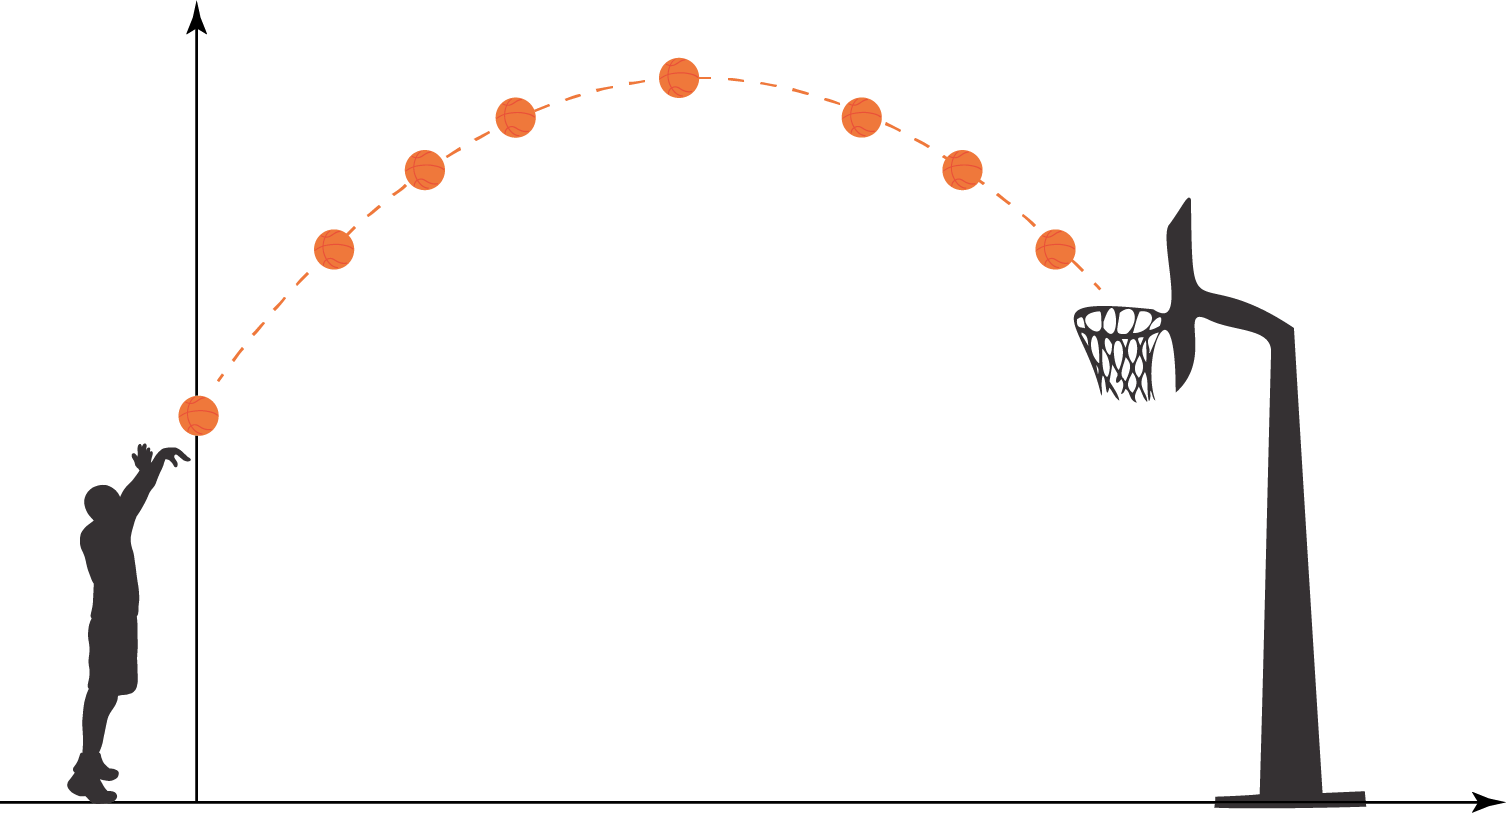
\includegraphics[width=\textwidth]{basquete}  
\end{center}

Admitindo que o jogador lançou a bola de uma altura de 2,10$m$ com velocidade inicial de $v_0 m/s$ (na direção vertical), a função que fornece a variação da altura da bola em função do tempo é dada pela expressão
\[h(t) = 2,10 + v_0 t - 5t^2\]
cujo gráfico também é uma parábola (representado a seguir apenas para $t\geq 0$):

\begin{figure}[H]
\centering
  \begin{tikzpicture}[xscale=2.8]
    \draw[help lines, thin, gray!30, step=.2] (0,0) grid (2.2,4.2);
    \draw[help lines, thin, gray!70] (0,0) grid (2.2,4.2);
    \draw [->, thick] (0,0) -- (0,4.4);
    \node[left, rotate=90] at (-.25,4) {altura (h)};
    \draw [->, thick] (0,0) -- (2.4,0);
    \node[] at (2,-.7) {tempo (t)};
    \foreach \x in {0.5,1,1.5,2} \draw (\x,.1)  -- (\x,-.1)  node[below] {\x};
    \foreach \y in {1,...,4} \draw (.03571,\y) -- (-.03571,\y) node[left] {\y};        
    \node[below left] at (0,0) {0};
    \draw [ domain=0:1.5, color=\currentcolor, smooth, very thick] plot (\x,-5*\x^2 +6*\x + 2.1);
  \end{tikzpicture}

\caption{Gráfico de $h(t)$ para $v_0 = 6m/s$.}
\end{figure}

Com a ajuda de uma calculadora, calcule as taxas de variação médias da altura nos seguintes intervalos de tempo para $v_0 = 6 m/s$ e $v_0 = 7 m/s$:

\begin{table}[H]
  \centering
\begin{tabu} to .7\textwidth{|l|c|c|}
  \hline
  \thead
          & $\bm{v_0 = 6 m/s}$ & $\bm{v_0 = 7 m/s}$ \\
\hline
Entre $t=0$ e $t=1$ & & \\
\hline
Entre $t=0$ e $t=0,1$ & & \\
\hline
Entre $t=0$ e $t=0,01$ & & \\
\hline
Entre $t=0$ e $t=0,001$ & & \\
\hline
Entre $t=0$ e $t=0,0001$ & & \\
\hline
\end{tabu}
\end{table}

\begin{enumerate}
\item Olhando para as sequências de valores obtidos acima, o que se pode conjecturar sobre a tendência que eles apresentam?

  Considerando a velocidade inicial igual a $6m/s$, a bola atinge sua altura máxima de $3,9m$ depois de $0,6s$ do lançamento. Ou seja, o ponto mais alto do gráfico é o par ordenado $(0{,}6;3{,}9)$. Neste ponto a velocidade na direção vertical é igual a zero (uma vez que aí a bola deixa de subir e passa a descer). Observe, agora, as taxas de variação médias da altura nos seguintes intervalos de tempo:


  \begin{multicols}{2}
    \begin{table}[H]
    \begin{tabu}[l]{|l|>{$}c<{$}|}
      \hline
      \tnumber
	  & \bm{v_0 = 6m/s} \\
      \hline
      Entre $t=0{,}5$ e $t=0{,}6$  & 0{,}5 \\
      \hline
      Entre $t=0{,}59$ e $t=0{,}6$  & 0{,}05 \\
      \hline
      Entre $t=0{,}599$ e $t=0{,}6$  & 0{,}005 \\
      \hline
      Entre $t=0{,}5999$ e $t=0{,}6$  & 0{,}0005 \\
      \hline
    \end{tabu}
\end{table}
\begin{table}[H]
    \begin{tabu}[r]{|l|c|}
      \hline
      \thead
      & $\bm{v_0 = 6m/s}$ \\
      \hline
      Entre $t=0{,}6$ e $t=0{,}7$  & -0,5 \\
      \hline
      Entre $t=0{,}6$ e $t=0{,}65$  & -0,25 \\
      \hline
      Entre $t=0{,}6$ e $t=0{,}605$  & -0,025 \\
      \hline
      Entre $t=0{,}6$ e $t=0{,}6005$  & -0,0025 \\
      \hline
    \end{tabu}
  \end{table}
\end{multicols}

  
\item A tendência observada nos valores obtidos acima corrobora a sua conjectura do item anterior? Explique.
\item Calcule a taxa de variação média da função $h(t) = 2,1 + 6t -5t^2$ entre os tempos $t=1$ e $t=1 + \alpha$, onde a variável $\alpha$ representa um número real próximo de zero. (A resposta ficará em função de $\alpha$).
  \item À medida que o valor de $\alpha$ se aproxima de zero, o que se observa com o valor da taxa de variação média calculada no item anterior? O que esse valor significa no contexto do problema?
  \end{enumerate}
\end{task}

  \exercise
\begin{answer}{Exercícios}
{\exerciselist
	\begin{enumerate}
	\item 
	\adjustbox{valign=t}
	{\setlength\tabcolsep{2.5pt}
	\setlength\tabulinesep{2.5pt}
	\begin{tabu}[l]{|c|c|c|}
	\hline
	\thead
	\makecell{Intervalo $\bm{[a,b]}$} & \makecell{Variação da função \\  $\bm{\Delta f = f(b) - f(a)}$} & \makecell{Variação média da função \\ $\bm{\dfrac{\Delta f}{\Delta x} = \dfrac{f(b) - f(a)}{b-a}}$} \\
	\hline
	$[-1,0]$ & $4$ & $4$\\
	\hline
	$[0,1]$ & $-1$ & $-1 $\\
	\hline
	$[1,2]$ & $2$ & $2$\\
	\hline
	$[-1,1]$ & $3$ & $\dfrac{3}{2}$ \\
	\hline
	$[0,2]$ & $1$ & $\dfrac{1}{2}$  \\
	\hline
	$[-1,2]$ & $5$ & $\dfrac{5}{2}$ \\
	\hline
    \end{tabu}
  	}
	\end{enumerate}
}{1}
\end{answer}
\clearmargin
\begin{answer}{Exercícios}
{\exerciselist
	\begin{enumerate}\setcounter{enumi}{1}
	\item 
	\begin{enumerate}
	\item $10$m/2 
	\item $-10$m/2
	\end{enumerate}
	\item $35{,}7$ reais por unidade
	\item
	\begin{enumerate}
	\item $8{,}29$
	\item $-1{,}33$
	\end{enumerate}
	\item 
	\begin{enumerate}
	\item $43$
	\item $95{,}5$
	\end{enumerate}

	\end{enumerate}
}{1}
\end{answer}
\clearmargin
\begin{answer}{Exercícios}
{\exerciselist
	\begin{enumerate}\setcounter{enumi}{5}
	\item A taxa de variação de $B$ para $C$ é maior do que a taxa de variação de $A$ para $C$, que é maior do que a taxa de variação de $A$ para $B$.
	\item Letra \textit{b)}
	\end{enumerate}
}{1}
\end{answer}
\clearmargin
\begin{answer}{Exercícios}
{\exerciselist
	\begin{enumerate}
	\item Letra \textit{d)}
	\end{enumerate}
}{1}
\end{answer}

  \begin{enumerate}
  \item Considere a função cujo gráfico está representado abaixo. Complete a tabela abaixo com as variações e as taxas de variação.

\begin{center}
\begin{tikzpicture}[domain=0:4, scale=1.3]
\draw[very thin,color=gray!50] (-2,-2) grid (3,5);
\draw[semithick](-2,0) -- (3,0);
\draw[semithick](0,-2) -- (0,5);

\node [below left] at (0,0) {0};

\draw[color=\currentcolor!80, domain=-1.10162:2.14327, samples=1000, smooth, very thick] plot (\x,{1.333333*(\x)^3-2.5*(\x)^2+0.166666*(\x)+3});

\foreach \x/\y in {-1/-1,0/3,1/2,2/4} \fill (\x,\y) circle (1.5pt);

\foreach \x in {-1,1,2} \node [below] at (\x,0) {\x};
\foreach \x in {-1,1,2,3,4} \node [left] at (0,\x) {\x};

\end{tikzpicture}
\end{center}

    
\begin{table}[H]
\centering
\setlength\tabulinesep{2.5pt}
\begin{tabu}[l]{|c|c|c|}
\hline
\thead
\makecell{Intervalo $\bm{[a,b]}$} & \makecell{Variação da função \\  $\bm{\Delta f = f(b) - f(a)}$} & \makecell{Variação média da função \\ $\bm{\dfrac{\Delta f}{\Delta x} = \dfrac{f(b) - f(a)}{b-a}}$} \\
\hline
$[-1,0]$ & & \\
\hline
$[0,1]$ & & \\
\hline
$[1,2]$ & & \\
\hline
$[-1,1]$ & & \\
\hline
$[0,2]$ & & \\
\hline
$[-1,2]$ & & \\
\hline
        \end{tabu}
      \end{table}

    \item (Velocidade Média) Se um objeto é arremessado para o alto a $20m/s$ a partir de uma altura de $6m$, sua altura $S$ após $t$ segundos é dada por
  \[S(t) = 6 + 20t - 5t^2.\]
  Qual é a velocidade média do objeto entre:
  \begin{enumerate}
  \item 0 e 2 segundos.
    \item 2 e 4 segundos.
    \end{enumerate}

    \item (Receita) A função que fornece a receita total em reais obtida com a venda de um determinado eletrodoméstico é
\[ R(x) = 36x - 0,01x^2,\]
em que $x$ é o número de unidades vendidas. Qual é a taxa da variação média da receita $R(x)$ à medida que $x$ aumenta de 10 para 20 unidades?

\item (Demanda) Se a demanda por um produto $p$ é dada pela função 
\[D(p) = \dfrac{1000}{\sqrt{p}} - 1, \]
  qual é a taxa de variação média da demanda quando p aumenta de

  \begin{enumerate}
  \item 1 para 25?
  \item 25 para 100?
  \end{enumerate}

\item (Custo total) Suponha que o custo total em dólares para a produção de $x$ impressoras seja dado pela função
  \[C(x) = 0,0001x^3 w + 0,005x^2 + 28x + 3000.\]
  Encontre a taxa de variação média do custo total quando a produção varia:
  \begin{enumerate}
  \item De 100 para 300 impressoras;
  \item De 300 para 600 impressoras.
  \end{enumerate}

\clearpage

\item A figura a seguir mostra o gráfico do custo total (em milhares de reais) em função da quantidade (em milhares de unidades) de um produto manufaturado por uma determinada companhia. Ordene, da menor para a maior, as taxas de variação médias do custo total de $A$ para $B$, $B$ para $C$ e $A$ para $C$.

  \begin{center}
%  \begin{tikzpicture}
%     \draw [->, thick] (0,-.5) -- (0,4.8) node[left] {$C(x)$};
%     \draw [->, thick] (-2.2,0) -- (3.2,0) node[below] {$x$};
%     \foreach \x in {2,4,...,10} \node[below] at (\x,0) {$10*\x$};
%     \foreach \y in {1,2,3,4,5} \node[left] at (0,\y) {$10*\y$};        
%     \draw [domain=-1.1:2.1, smooth, color=\currentcolor, thick] plot (\x, sin\x^3 -2x^2+ 3);
% \foreach \x / \y in {2.1/0.9, 4/1.8, 6/3.7}  \fill (\x,\y) circle (3pt);
%     \end{tikzpicture}
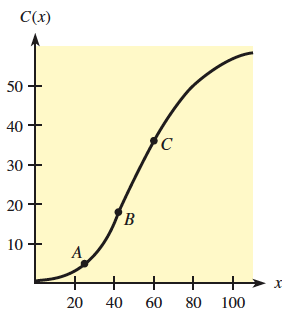
\includegraphics[width=.3\textwidth]{taxa-exerc-6}
  \end{center}

\item (ENEM 2019) Os exercícios físicos são recomendados para o bom funcionamento do organismo, pois aceleram o metabolismo e, em consequência, elevam o consumo de calorias. No gráfico, estão registrados os valores calóricos, em kcal, gastos em cinco diferentes atividades físicas, em função do tempo dedicado às atividades, contado em minuto.

\begin{figure}[H]
\centering
\begin{tikzpicture}[yscale=.25, scale=1, every node/.style={scale=.9}]

\draw [thick] (0,0) -- (6,0) node [below, pos=1.1] {Tempo (min)};
\draw [thick] (0,0) -- (0,14);

\foreach \x/\y in {0/5,1/10,2/15,3/20,4/25,5/30,6/\phantom{a}} 
{\draw [gray!70] (\x,0) -- (\x,14);
\node [below] at (\x,0) {\y};};

\node [rotate=90, above] at (-.75,7) {(kcal)};

\foreach \y in {2,4,...,14} 
{\draw [gray!70] (0,\y) -- (6,\y);
\node [left] at (0,\y) {\y0};};

\foreach \x/\y/\z in {1/2/I,2/10/II,3/12/III,4/10/IV,5/8/V}
{\node [circle, fill, inner sep=2pt, label=above right:\z] at (\x,\y) {};};

\end{tikzpicture}
\end{figure}

  Qual dessas atividades físicas proporciona o maior consumo de quilocalorias por minuto?

  \begin{enumerate}
  \item I
  \item II
  \item III
  \item IV
  \item V
  \end{enumerate}

\clearpage

\item (ENEM 2019) O gráfico a seguir mostra a evolução mensal das vendas de certo produto de julho a novembro de 2011.

  \begin{center}
\begin{tikzpicture}[scale=.75, every node/.style={scale=1}, xscale=1.5]

\draw [->] (0,0) -- (0,6.5) node [above left, align=center] {Unidades \\ vendidas};
\draw [->] (0,0) -- (6,0);

\foreach \x/\y in {.7*2/700,2.3*2/2.500,2.7*2/2.700,3*2/2.800} \node [left] at (0,\x) {\y};

\foreach \x/\y in {1/Jul,2/Ago,3/Set,4/Out,5/Nov,6/Mês} \node [below] at (\x,0) {\y};

\foreach \x/\y in {(1,.7*2)/a,(2,2.3*2)/b,(3,2.3*2)/c,(4,3*2)/d,(5,2.7*2)/e} \node (\y) [coordinate] at \x {};

\draw [dashed] (0,.7*2) -- (a) -- (1,0);
\draw [dashed] (0,2.3*2) -- (b) -- (2,0);
\draw [dashed] (0,2.3*2) -- (c) -- (3,0);
\draw [dashed] (0,3*2) -- (d) -- (4,0);
\draw [dashed] (0,2.7*2) -- (e) -- (5,0);

\draw [very thick, \currentcolor!80] (a) -- (b) -- (c) -- (d) -- (e);
\end{tikzpicture}   
  \end{center}

  
  Sabe-se que o mês de julho foi o pior momento da empresa em 2011 e que o número de unidades vendidas desse produto em dezembro de 2011 foi igual à média aritmética do número de unidades vendidas nos meses de julho a novembro do mesmo ano. O gerente de vendas disse, em uma reunião da diretoria, que, se essa redução no número de unidades vendidas de novembro para dezembro de 2011 se mantivesse constante nos meses subsequentes, as vendas só voltariam a ficar piores que julho de 2011 apenas no final de 2012. O diretor financeiro rebateu imediatamente esse argumento mostrando que, mantida a tendência, isso aconteceria já em

  \begin{enumerate}
  \item Janeiro
  \item Fevereiro
  \item Março
  \item Abril
  \item Maio
  \end{enumerate}
\end{enumerate}